\documentclass[11pt]{article}

% Change "review" to "final" to generate the final (sometimes called camera-ready) version.
% Change to "preprint" to generate a non-anonymous version with page numbers.
\usepackage[preprint]{acl}

% Standard package includes
\usepackage{times}
\usepackage{latexsym}
\usepackage[T1]{fontenc}
\usepackage[utf8]{inputenc}
\usepackage{microtype}
\usepackage{inconsolata}
\usepackage{graphicx}
\usepackage{fontawesome5}

% Colors used in the author block (links / icons)
\definecolor{darkblue}{HTML}{0E4D92}

% Additional packages used by sections / appendix (carried over from the ACM template)
\usepackage{xurl}
\usepackage{booktabs}
\usepackage{float}
\usepackage{amsmath}
\usepackage{amsfonts}
\usepackage{array}
\usepackage{colortbl}
\usepackage{tabularx}
\usepackage{makecell}
\usepackage{tikz}
\usepackage{pgfplots}
\pgfplotsset{compat=1.18}
\usetikzlibrary{shapes.geometric, arrows.meta, positioning, calc, backgrounds, fit, shadows}
\usepackage[most]{tcolorbox}

% Monospace identifiers that may exceed column width (breaks at `-`, `_`, etc.; no hyperlink).
\newcommand{\skillcode}[1]{\begingroup\urlstyle{tt}\nolinkurl{#1}\endgroup}
\newcommand{\skillfile}{\texttt{skill specification }}
\newcommand{\skillpackage}{skill package}
\newcommand{\skillpackages}{skill packages}

% Appendix / supplementary styling (olive header, cream body; matches prompt-table aesthetic)
\definecolor{appendixolive}{HTML}{8B8B5E}
\definecolor{appendixcream}{HTML}{FDFCF0}
\newcommand{\apdxhdr}[1]{\textcolor{white}{\textbf{#1}}}

\newtcolorbox{ApdxTabFrame}[1][]{%
  enhanced,
  sharp corners,
  arc=0pt,
  boxrule=0.55pt,
  colframe=appendixolive,
  colback=appendixcream,
  left=5pt,
  right=5pt,
  top=5pt,
  bottom=5pt,
  width=\linewidth,
  #1,
}

\newtcblisting{GosPromptBox}[1]{%
  enhanced,
  sharp corners,
  arc=0pt,
  boxrule=0.55pt,
  colframe=appendixolive,
  colback=appendixcream,
  colbacktitle=appendixolive,
  coltitle=white,
  fonttitle=\bfseries\sffamily\footnotesize,
  titlerule=0mm,
  boxsep=3pt,
  left=8pt,
  right=8pt,
  top=2pt,
  bottom=6pt,
  title={#1},
  listing only,
  listing engine=listings,
  listing options={%
    basicstyle=\ttfamily\footnotesize,
    breaklines=true,
    columns=fullflexible,
    keepspaces=true,
    aboveskip=0pt,
    belowskip=0pt,
    xleftmargin=0pt,
  },
}

\newtcolorbox{ApdxCallout}[1][]{%
  enhanced,
  sharp corners,
  arc=0pt,
  boxrule=0.55pt,
  colframe=appendixolive,
  colback=appendixcream,
  fontupper=\small,
  left=8pt,
  right=8pt,
  top=6pt,
  bottom=6pt,
  #1,
}

% Algorithm float + box used by the appendix pseudocode
\floatstyle{plain}
\newfloat{algorithm}{t}{loa}
\floatname{algorithm}{Algorithm}
\captionsetup[algorithm]{font=small,labelfont=bf}

\newenvironment{algobox}{%
  \begin{tcolorbox}[
    enhanced,
    sharp corners,
    arc=0pt,
    boxrule=0.55pt,
    colframe=appendixolive,
    colback=appendixcream,
    fontupper=\small,
    left=8pt,
    right=8pt,
    top=8pt,
    bottom=8pt,
  ]
}{%
  \end{tcolorbox}
}

\newcommand{\alginput}[1]{\textbf{Input:} #1\\}
\newcommand{\algoutput}[1]{\textbf{Output:} #1\\}
\newcommand{\algstep}[1]{#1\\}
\newcommand{\algindent}[1]{\hspace*{1.5em}#1\\}

\title{Graph-of-Skills: Dependency-Aware Structural Retrieval for Massive Agent Skills}

% Non-anonymous author block for arXiv preprint.
\author{Dawei Liu\textsuperscript{1}\thanks{Core Contribution.} \quad Zongxia Li\textsuperscript{2}\footnotemark[1] \quad Hongyang Du\textsuperscript{3} \quad Xiyang Wu\textsuperscript{2} \quad Shihang Gui\textsuperscript{3}\\ \textbf{Yongbei Kuang}\textsuperscript{4} \quad \textbf{Lichao Sun}\textsuperscript{5}\\[0.5ex] \textsuperscript{1}University of Pennsylvania \quad \textsuperscript{2}University of Maryland  \quad \textsuperscript{3}Brown University \quad \\\textsuperscript{4}Carnegie Mellon University  \quad \textsuperscript{5}Lehigh University \\ {\tt\small liudawei@seas.upenn.edu \quad zli12321@umd.edu \quad lis221@lehigh.edu} \\[0.4ex] \makebox[\textwidth][c]{\small
  \href{https://github.com/davidliuk/graph-of-skills}{\textcolor{darkblue}{\faIcon{github}}}\kern0.35em
  \textbf{Code:}\kern0.35em
  \url{https://github.com/davidliuk/graph-of-skills}} }

\begin{document}
\maketitle

\begin{abstract}
Modern LLM agents increasingly rely on reusable skills, and as they interact with personal applications, web browsers, and other interfaces, skill libraries can scale to thousands of skills.
% ~\citep{patil2023gorilla, li2023apibank, qin2024toolllm}.
%
Scaling to larger skill sets introduces two key challenges. First, loading the full skill set saturates the context window, driving up token costs, hallucination, and latency. Second, semantic retrieval surfaces topically relevant skills but misses their prerequisite chain of upstream and downstream skills, creating a prerequisite gap that leaves the retrieved bundle execution-incomplete.
% ~\citep{agentskills2026, liu-etal-2024-lost}. 
% the full skill set saturates the context window, driving up token costs, hallucination, and latency. 
% the bottleneck shifts from \emph{skill authoring} to \emph{reusable skill retrieval}: organizing skills into hierarchical, easily traversable structures so that only the most relevant subset actually needed for execution is loaded into context to complete tasks.
%
% Flat skill loading saturates the context window and inflates both token cost and latency. Vector retrieval surfaces semantically similar skills but often misses the parsers, preprocessors, and setup utilities they depend on---the \textit{Prerequisite Gap}.
%
In this paper, we present \textbf{Graph-of-Skills (GoS)}, an inference-time structural retrieval layer for large skill libraries.
%
GoS constructs an executable skill graph offline from skill packages, then at inference time retrieves a bounded, dependency-aware skill bundle through hybrid semantic--lexical seeding, reverse-aware Personalized PageRank, and context-budgeted hydration.
%
On SkillsBench and ALFWorld, GoS consistently delivers substantial reward improvements and token savings across three model families (Claude Sonnet 4.5, MiniMax M2.7, and GPT-5.2 Codex). 
%
On SkillsBench, GoS achieves a peak reward increase of $25.55\%$ while reducing total tokens by $56.72\%$ over the vanilla full skill-loading baseline using GPT-5.2 Codex.
%
Ablations confirm this pattern across skill libraries from 200 to 2{,}000 skills.
%
% Additional ablation studies show that semantic--lexical seeding and Personalized PageRank

\end{abstract}


\section{Introduction}
%
Large Language Model (LLM) agents solve complex technical tasks by invoking external tools, APIs, and reusable skills \citep{schick2023toolformer, mialon2023augmented}. 
%
As these tools and skills grow from dozens of tools to thousands or even tens of thousands of candidates \citep{patil2023gorilla, li2023apibank, xu2023toolbench, qin2024toolllm}, the core challenge shifts from deciding \emph{whether} to use a skill to retrieving the most relevant set of skills that is sufficient for a task. 
%
\citet{shi2025toolret} already shows that skill retrieval itself is now a major bottleneck in realistic tool ecosystems.

Two common strategies are widely used for handling large skill libraries. 
%
\textbf{Vanilla Skills}~\citep{agentskills2026} prepends the entire skill set to the context window. 
%
This can work for small toolsets, but it scales poorly: token cost grows linearly with library size, and critical domain constraints become easy for the model to overlook inside an overloaded context \citep{liu-etal-2024-lost}.
%\textcolor{red}{cite the paper: lost in the middle}. 
An alternative is \textbf{vector-based retrieval} \citep{lewis2020retrieval, wang2023voyager}, which improves efficiency by retrieving semantically similar skills. 
%
However, semantic proximity does not imply executable sufficiency. In many engineering tasks, the top semantic match is a high-level solver, while the actual solution also requires a lower-level parser, converter, setup utility, or domain-specific preprocessor that is semantically weak but functionally necessary~\citep{qin2024toolllm, liu2025dynamic, patil2023gorilla} (Figure~\ref{fig:prerequisite_gap}).

\begin{figure*}[!t]
    \centering
    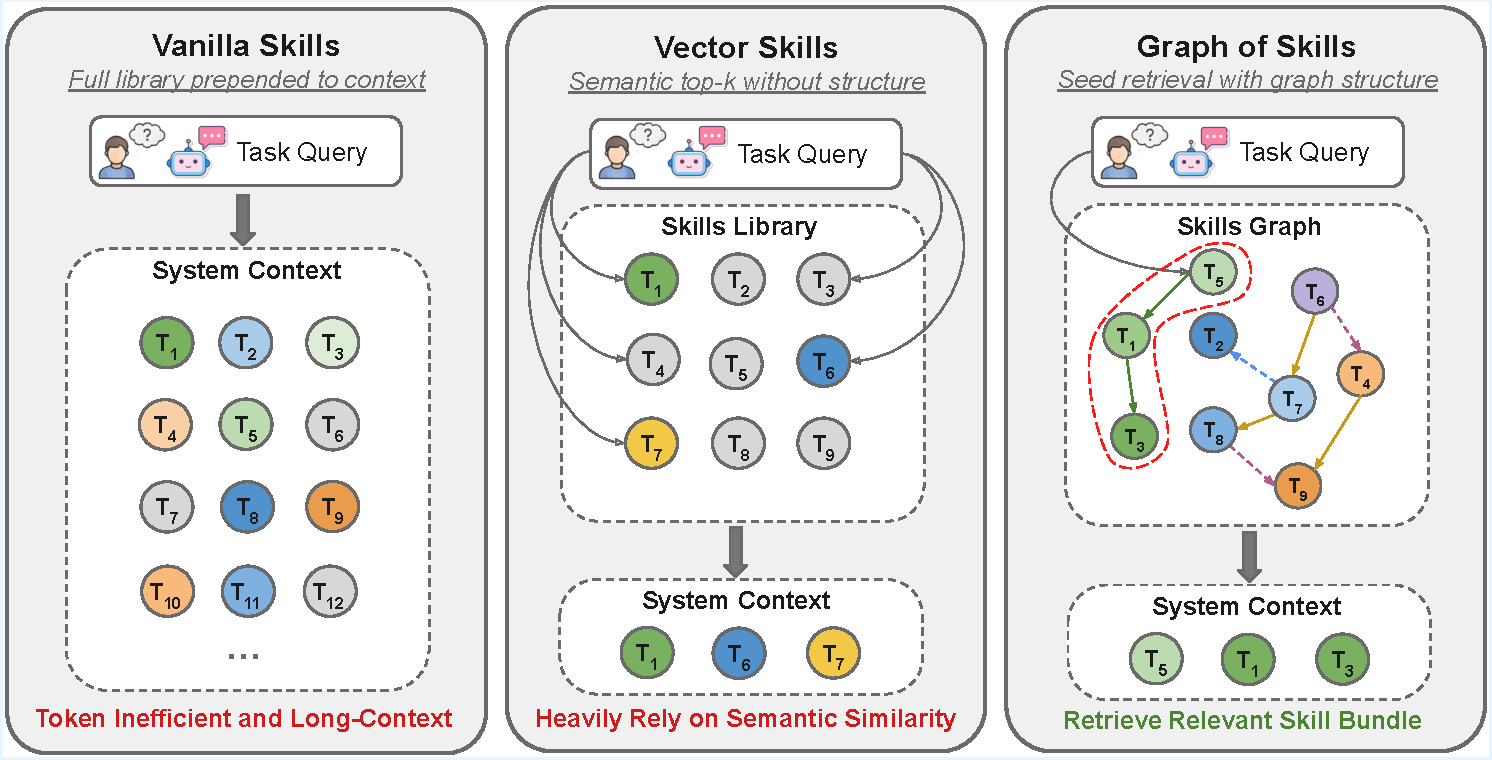
\includegraphics[width=\textwidth]{assests/compare.pdf}
    \caption{Conceptual comparison between flat skill loading, vector retrieval, and Graph-of-Skills (GoS). \textbf{Vanilla Skills} prepends the full skill library to the prompt, so relevant constraints and prerequisite skills become buried in an overloaded context. \textbf{Vector Skills} improves efficiency by returning semantically similar skills, but it can still miss a functionally required prerequisite outside the retrieved set, creating the prerequisite gap. \textbf{Graph-of-Skills} starts from hybrid semantic-lexical seeds and then performs structure-aware retrieval to recover prerequisite skills and assemble a compact execution bundle.}
    \label{fig:prerequisite_gap}
\end{figure*}

% \vspace{-10pt}

We present \textbf{Graph-of-Skills} (GoS), an inference-time structural retrieval layer for large local skill libraries to combat limitations of the previous two approaches. GoS constructs a directed multi-relational graph over local skill packages, where nodes are executable skills and edges encode prerequisite and workflow structure. At query time, GoS uses semantic and lexical signals only to identify a small seed set, then applies reverse-aware Personalized PageRank (PPR)~\citep{10.1145/511446.511513, 10471277} to recover additional skills that are structurally important for execution. The result is a bounded skill bundle that is both relevant and closer to dependency-complete than isolated top-$k$ retrieval.
%
This setting is complementary to repository-scale skill infrastructures such as SkillNet and AgentSkillOS~\citep{skillnet2026, li2026agentskillos}, which focus on creating, organizing, and orchestrating large skill ecosystems. GoS instead targets the downstream question: given an existing local skill library, how should an agent retrieve the smallest executable subset sufficient for the current task? It parses each \skillfile into executable fields, constructs typed dependency and workflow edges, and retrieves a bounded bundle through graph diffusion plus reranking.

Our contributions are as follows:
    % \item We define the \textit{Prerequisite Gap}, a retrieval failure mode in which the semantically obvious skill is found but the executable prerequisite chain is omitted.
    (1) We introduce GoS, an agentic skill usage pipeline that combines offline graph construction with inference-time structural retrieval to improve skill selection accuracy while reducing input token consumption.
    (2) We evaluate GoS across two benchmarks (SkillsBench, ALFWorld) and three model families, and find that on the 1{,}000-skill SkillsBench setting under GPT-5.2 Codex, GoS attains a peak reward gain of 25.55\% over the full skill-loading baseline while reducing total tokens by 56.72\%, with consistent improvement over both baselines in every model--benchmark block. Additional ablations confirm this pattern across skill libraries from 200 to 2{,}000 skills.

\section{Related Work}

\noindent\textbf{Tool Use, Tool Discovery, and Tool Retrieval for Agents.}
%
Early research on tool-augmented language models focuses on relatively small, fixed toolsets, where the primary challenge is deciding \emph{when} to invoke a tool and formatting the call correctly~\citep{schick2023toolformer, mialon2023augmented}.
%
As tool sets grow from dozens of tools to thousands~\citep{patil2023gorilla, li2023apibank, xu2023toolbench, qin2024toolllm} and context windows continue to expand~\citep{singh2025openai,li2026mm, comanici2025gemini}, the problem shifts toward \emph{tool discovery} and \emph{tool retrieval}. Systems and benchmarks such as Gorilla~\cite{patil2023gorilla}, API-Bank~\cite{li2023apibank}, ToolBench-style evaluations~\cite{xu2023toolbench}, and ToolLLM~\cite{qin2024toolllm} show that large tool universes require scalable retrieval over API descriptions and tool documentation.
%
ToolNet \citep{liu2024toolnet} introduces graph structure into large-scale tool access, with the objective to connect models to broad tool ecosystems rather than recover dependency-complete local executable bundles. 
%
However, \citet{shi2025toolret} shows that tool retrieval is itself a difficult modeling problem and that generic dense retrievers are often poorly aligned with real tool-use needs \citep{shi2025toolret}. 
%
% GoS builds on this literature but targets a different failure mode: the semantically nearest skill may be retrieved while the supporting prerequisite chain is omitted.

% \noindent\textbf{Experience Consolidation and Skill Acquisition.} A parallel line of work studies how agents acquire reusable skills, memories, and abstractions from prior interaction. Reflexion \citep{reflexion2023} and ExpeL \citep{zhao2024expel} show that agents can summarize failures and reuse verbalized experience. Voyager \citep{wang2023voyager} demonstrates open-ended skill accumulation in embodied environments. More recent work studies programmatic or agent-induced skill formation, including SkillWeaver \citep{zheng2025skillweaver}, ASI \citep{wang2025asi}, and CUA-Skill \citep{chen2026cuaskill}. These methods primarily expand, refine, or transfer a skill set over time. GoS is complementary: it assumes a local skill corpus already exists and asks how an agent should retrieve from that corpus efficiently at inference time. In this sense, skill-acquisition methods grow the repository, whereas GoS structures and traverses it to recover the smallest executable subset for a given task.

\noindent\textbf{Agent Skills Ecosystems.} Recent systems increasingly treat agent skills as reusable assets rather than ad hoc prompts~\citep{agentskills2026, skillnet2026, li2026agentskillos}.
%
SkillNet~\citep{skillnet2026} and AgentSkillOS~\citep{li2026agentskillos} advocate ecosystem-level approaches emphasizing systematic categorization, ontology construction, and dynamic chaining over large skill collections, while SkillsBench~\citep{li2026skillsbench} shows that curated external skills can improve agent performance but having many skills available does not guarantee reliable use.
%
Adjacent registries such as SkillsMP, ClawHub, and LangSkills similarly support packaging, discovery, and search over large skill collections~\citep{skillsmp2026, clawhub2026, li2025self,langskills2026}, but their primary interface remains entry-level search or distribution over individual skills or bundles.
% GoS instead targets the downstream inference-time problem of recovering a small bundle that is not only relevant, but also structurally sufficient for execution.


\noindent\textbf{Graph-Based Retrieval and Relational Memory.} 
Graph-structured retrieval has recently improved knowledge access in document, memory, and tool-use settings, but its role differs substantially across these regimes. GraphRAG \citep{edge2024graphrag} uses graph structure to support query-focused synthesis over document collections, HippoRAG \citep{gutierrez2024hipporag} models long-term memory as an associative graph for improved retrieval, and adjacent agent systems such as ControlLLM \citep{liu2023controlllm} and ToolNet \citep{liu2024toolnet} incorporate graph structure over tools rather than treating tools as a flat list.
%
However, these lines of work do not directly study retrieval over large local skill repositories. GraphRAG-style systems target knowledge synthesis, memory access, or relational QA; tool-graph methods focus primarily on graph-guided tool planning and navigation during reasoning. By contrast, our setting requires an \emph{upstream} retrieval layer that selects a small executable bundle \textit{before} generation begins. To our knowledge, prior work has not focused on graph-based retrieval for agent skills under this objective: recovering a dependency-complete executable bundle under a tight context budget, rather than merely retrieving one relevant item.

% whereas GoS focuses on inference-time retrieval of a bounded local skill bundle for general-purpose coding and technical tasks. The shared intuition is that retrieval should exploit relations, but agent skills impose an additional operational constraint: the retrieved items must not only be relevant, but also \emph{jointly executable}. This motivates our use of a typed, directed skill graph with reverse-aware diffusion over dependency edges.


\section{Methodology}
\label{sec:methodology}

\begin{figure*}[!t]
    \centering
    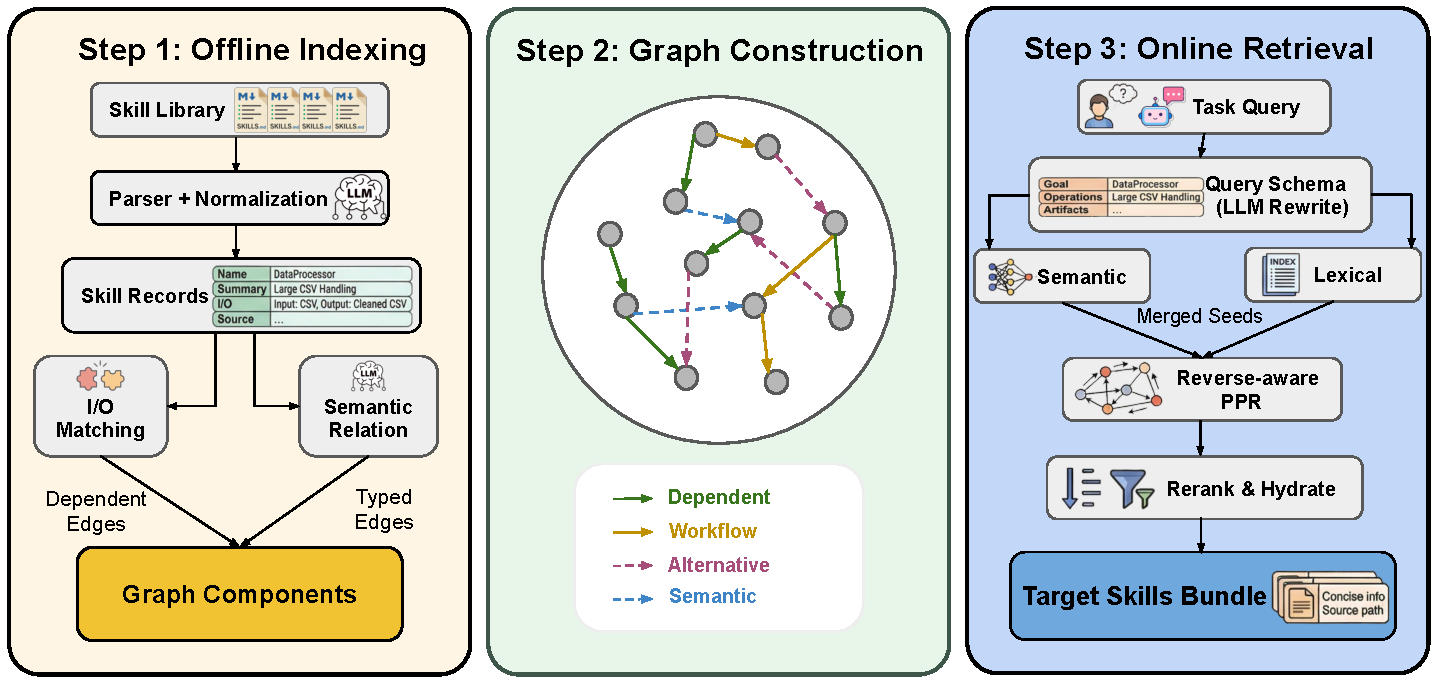
\includegraphics[width=1\linewidth]{assests/arch.pdf}
    \caption{Overview of Graph of Skills (GoS). \textbf{Left:} offline indexing converts local \skillpackages{} into normalized skill records and typed edges. Dependency edges are induced from I/O compatibility, while workflow, semantic, and alternative relations are added through sparse validation. \textbf{Center:} the typed directed skill graph is the retrieval substrate; edge labels denote dependency, workflow, semantic, and alternative relations. \textbf{Right:} online retrieval maps a task query to a compact query schema, forms merged seeds from semantic and lexical retrieval, applies reverse-aware Personalized PageRank, and returns a budgeted execution bundle after reranking and hydration.}
    \label{fig:gos_arch_horizontal}
\end{figure*}

GoS is an inference-time retrieval layer for large local skill libraries. It constructs a typed graph offline from local \skillpackages{} and, at query time, returns a compact execution bundle that is relevant to the task and more likely than flat retrieval to include the prerequisites required for successful execution.

\subsection{Problem Setup}
Let $\mathcal{C} = \{d_1, \dots, d_m\}$ denote a local corpus of \skillpackages{}. Each package contains a primary specification document together with optional scripts, references, and auxiliary assets. GoS converts $\mathcal{C}$ into a typed directed graph
\begin{equation}
    G = (V, E, w, \phi),
\end{equation}


where each node $v \in V$ is a normalized executable skill record, each edge $e \in E$ connects two skills, $w(e) > 0$ is an edge weight, and $\phi(e) \in \mathcal{R}$ assigns an edge type from the relation set
\begin{equation}
\mathcal{R} = \{\mathrm{dep}, \mathrm{wf}, \mathrm{sem}, \mathrm{alt}\}.
\end{equation}

Given a task query $q$ and a context budget $\tau$, the retrieval problem is to return a bundle $B(q) \subseteq V$ that is simultaneously relevant, execution-complete when possible, and compact. We view this as a budgeted selection problem,
% \begin{equation}
% \begin{aligned}
% \max_{B \subseteq V} \; & \sum_{v \in B} \operatorname{rel}(v, q) \\
% & + \beta \!\!\!\!\sum_{(u,v) \in E_{\mathrm{dep}}} \!\!\!\!\mathbb{I}[u \in B \wedge v \in B] \\
% & \text{s.t.} \; \operatorname{cost}(B) \le \tau,
% \end{aligned}
% \label{eq:objective}
% \end{equation}
\begin{equation}
\begin{aligned}
\max_{B \subseteq V} \; & \sum_{v \in B} \operatorname{rel}(v, q) + \beta \!\!\!\!\sum_{(u,v) \in E_{\mathrm{dep}}} \!\!\!\!\mathbb{I}[u \in B \wedge v \in B] \\
& \text{s.t.} \quad \operatorname{cost}(B) \le \tau
\end{aligned}
\label{eq:objective}
\end{equation}
where the first term favors query relevance, the second rewards dependency-complete bundles, and $\operatorname{cost}(B)$ measures the prompt budget consumed by the hydrated bundle. Equation~\eqref{eq:objective} is not solved exactly. Instead, GoS approximates this objective through three stages: hybrid seed retrieval, reverse-aware graph diffusion, and budgeted reranking plus hydration.

\subsection{Offline Graph Construction}
\noindent\textbf{Skill Normalization.}
Each \skillpackage{} is parsed into a normalized skill record containing a canonical name, capability summary, I/O fields, domain tags, tooling, entrypoints, compatibility notes, and a stable local source path. This normalization step is primarily deterministic: the system extracts executable fields whenever possible and uses a lightweight LLM pass only to recover retrieval-critical semantic fields when package documentation is incomplete. The goal is to convert each local skill into a retrieval unit that an agent can directly consume at inference time.

\noindent\textbf{Typed Relation Induction.}
GoS uses four edge types. \emph{Dependency} edges represent executable prerequisites and form the primary structural relation in the graph. A dependency edge $v_i \rightarrow v_j$ is added \emph{deterministically} whenever the I/O schemas of $v_i$ and $v_j$ overlap above a fixed threshold, so that $v_i$ can plausibly provide an artifact consumed by $v_j$; no LLM call is involved. \emph{Workflow} edges capture common multi-step pipelines, \emph{semantic} edges connect near-duplicate or topically adjacent skills, and \emph{alternative} edges link interchangeable strategies for the same subproblem.

Rather than performing unconstrained all-pairs relation inference, GoS constructs the three non-dependency edge types through sparse LLM validation. For each node, it first forms a small candidate pool using lexical similarity, semantic neighbors, and I/O-based expansion, and only the top-$k$ candidates per node are submitted to a constrained validator prompt (default $k{=}8$). Total LLM validation calls therefore scale as $\mathcal{O}(N k)$ rather than $\mathcal{O}(N^2)$, and incremental indexing further reduces this to $\mathcal{O}(|V_{\mathrm{new}}|\,N)$. This keeps graph construction tractable while anchoring the resulting graph in executable structure rather than metadata proximity alone.

\subsection{Online Structural Retrieval}
\noindent\textbf{Query Representation and Hybrid Seeding.}
Dense retrieval~\citep{karpukhin2020dense} is often effective at finding the visible top-level skill but weak at recovering semantically subtle prerequisites. Lexical retrieval in the probabilistic ranking tradition~\citep{robertson2009probabilistic} is robust for concrete artifacts and filenames, but brittle under paraphrase. GoS therefore combines the two signals at the seeding stage.

At retrieval time, the raw query is mapped to a lightweight retrieval schema containing the task goal, salient operations, referenced artifacts, and normalized keywords. This schema can be produced by an optional LLM rewrite, following the general intuition of rewrite-then-retrieve pipelines~\citep{ma2023query}; when rewriting is unavailable or disabled, GoS falls back to deterministic lexical normalization. GoS then computes a semantic seed score $s_i^{\mathrm{sem}}(q)$ and a lexical seed score $s_i^{\mathrm{lex}}(q)$ for each candidate skill $v_i$, and merges them as
\begin{equation}
 z_i(q) = \eta \, s_i^{\mathrm{sem}}(q) + (1-\eta) \, s_i^{\mathrm{lex}}(q),
 \label{eq:seed}
\end{equation}
where $\eta \in [0,1]$ controls the semantic--lexical tradeoff. The initial seed distribution is obtained by normalizing the merged scores over the candidate pool,
\begin{equation}
\mathbf{p}_i = \frac{z_i(q)}{\sum_j z_j(q)}.
\end{equation}

\noindent\textbf{Reverse-Aware Typed Diffusion.}
Let $A_r$ denote the weighted adjacency matrix for relation type $r \in \mathcal{R}$. To let retrieval move from a matched high-level skill toward likely prerequisites, GoS uses both forward and reverse transitions. For each relation type, we define a row-normalized forward operator $T_r^{\rightarrow}$ and a row-normalized reverse operator $T_r^{\leftarrow}$ obtained from $A_r$ and $A_r^{\top}$, respectively. GoS then forms the unified transition operator
\begin{equation}
T = \operatorname{RowNorm}\!\left( \sum_{r \in \mathcal{R}} \lambda_r \left(T_r^{\rightarrow} + \gamma_r T_r^{\leftarrow}\right) \right),
\label{eq:transition}
\end{equation}
where $\lambda_r \ge 0$ and $\sum_r \lambda_r = 1$ weight relation types, and $\gamma_r \ge 0$ controls how strongly reverse traversal is allowed for each type. In practice, reverse edges are inserted directly into the transition matrix with type-specific weights (largest for dependency, smallest for alternative; concrete values in Appendix~\ref{tab:appendix_relation_weights}), and the matrix is row-normalized before diffusion.

The core retrieval step is a reverse-aware Personalized PageRank-style diffusion over this operator~\citep{page1999pagerank, jeh2003scaling, 10471277}:
\begin{equation}
\mathbf{s}^{(\ell+1)} = \alpha \, \mathbf{p} + (1-\alpha) T^{\top} \mathbf{s}^{(\ell)},
\label{eq:ppr}
\end{equation}
where $\alpha \in (0,1)$ is the restart parameter. Relative to flat top-$k$ retrieval, relevance is not assigned only to individually matched skills; it is propagated across a local executable neighborhood. In particular, once a high-level solver is retrieved as a seed, upstream parser, setup, or preprocessing skills can still accumulate score through reverse dependency paths even when they are not themselves strong semantic matches to the original query.

\noindent\textbf{Budgeted Reranking and Hydration.}
The diffusion score alone is insufficient, because the final output must be compact and directly usable by an agent. GoS therefore reranks candidate skills by combining graph score with field-level query evidence:
\begin{equation}
\rho_i(q) = \mathbf{s}_i^{\star} + \mu \, m_i(q),
\label{eq:rerank}
\end{equation}
where $\mathbf{s}_i^{\star}$ is the converged diffusion score, $m_i(q)$ aggregates direct matches between the query and skill fields such as name, capability summary, artifacts, and entrypoints, and $\mu$ controls how much local grounding is preserved after graph expansion.

Candidates are then hydrated in descending order of $\rho_i(q)$ under both per-skill and global context budgets. Here, \emph{hydration} denotes materializing a selected skill into an agent-consumable payload that includes a stable source path together with concise capability text and the most relevant execution notes. The final output is therefore a bounded execution bundle designed to maximize executable coverage within the prompt budget.


% GoS' central design choice is to cast retrieval as a structured bundle-selection problem: semantic and lexical matching identify promising entry points, graph diffusion recovers missing prerequisites, and budgeted hydration enforces compactness. This combination allows GoS to improve task reward while preserving the efficiency benefits of retrieval.


\section{Experiments}
We evaluate whether graph-structured retrieval improves agent performance and efficiency relative to flat full-library access and non-graph semantic retrieval.


\subsection{Experimental Setup}
We evaluate GoS on two benchmarks using the full released task sets.
%
\textbf{SkillsBench}~\citep{li2026skillsbench} contains a diverse set of real-world technical tasks across 11 domains, paired with curated Skills: structured packages of procedural knowledge (instructions, code templates, resources) that augment LLM agents at inference time.
%
The task domains span complex technical work such as macroeconomic detrending, power-grid feasibility analysis, 3D scan analysis, financial modeling, and seismic phase picking.
%
%
\textbf{ALFWorld}~\citep{shridhar2020alfworld} is an interactive simulator that aligns text descriptions and commands with a physically embodied robotic environment, built by combining TextWorld~\citep{cote2018textworld}, an engine for interactive text-based games and the ALFRED dataset~\citep{shridhar2020alfred}.
%
Its tasks involve multi-step household activities such as navigating rooms, finding objects, and manipulating them.
%
In the LLM agent literature, ALFWorld is widely used in its text-only mode as a benchmark for sequential decision making, where an agent receives textual room descriptions and must issue a chain of commands to accomplish a goal~\citep{yao2023react, reflexion2023}. We evaluate on the full 140 episodes.


\noindent\textbf{Baselines.}
%
We compare GoS against two baselines.
%
\textit{Vanilla Skills} exposes the entire skill library directly to the agent, maximizing recall but providing no retrieval-time compression. On ALFWorld, this follows the official Agent Skills format and reference repository~\citep{agentskills2026}.
%
\textit{Vector Skills} retrieves a bounded set of skills using semantic similarity over the same embedding model used by GoS, namely \skillcode{openai/text-embedding-3-large}~\citep{openai2024textembedding3large} (3072 dimensions). It isolates the effect of graph structure from the general benefit of retrieval-time compression.
%
\textit{GoS} uses the same base embedding model as \textit{Vector Skills} but replaces flat nearest-neighbor retrieval with structure-aware retrieval over the skill graph. We disable the optional query-rewrite module so that any observed gain can be attributed to graph propagation rather than to an LLM rewrite of the query, and use the raw task instruction as the retrieval query. The critical comparison is therefore between flat semantic retrieval and dependency-aware structural retrieval under the same backbone and embedding setup.


\noindent\textbf{Models and Evaluation.}
Experiments are conducted with Claude Sonnet 4.5~\citep{anthropic2025claude45}, MiniMax M2.7~\citep{minimax2026m27}, and GPT-5.2 Codex~\citep{openai2025gpt52codex}.
%
Each model--method setting is run twice, and we report the mean across runs. We report average reward across tasks as the primary evaluation metric. For ALFWorld, rewards are binary, so average reward is equivalent to success rate. We additionally report average total token usage and agent-only runtime; runtime is measured from agent start to agent finish and excludes environment setup.


\noindent\textbf{Evaluation Protocol.}
We use the full benchmark task sets and apply the same retry policy across the main and sensitivity experiments. If environment construction fails, we rebuild and rerun the task up to two additional times; tasks that still fail after these retries are excluded as unresolved infrastructure failures rather than counted as model failures. For agent timeouts, we distinguish between substantive execution failures and startup failures: if the agent has already been executing for a long time and then times out, we record reward $0$ and keep the run in the aggregate; if the timeout occurs before a meaningful run is established, we rerun the trial. This protocol is applied to the full SkillsBench evaluation, the full 140-episode ALFWorld evaluation, and the library-size sensitivity study.


\subsection{Main Results}

We present the main results in Table~\ref{results-table}.
%
Across all six model--benchmark blocks, GoS attains the highest average reward. Relative to \textit{Vanilla Skills}, it reduces average token usage in all six blocks and reduces agent runtime in five of the six. Relative to \textit{Vector Skills}, it improves reward in every block while keeping the token budget in the same compressed regime.

\begin{table*}[t]
\caption{\textbf{R} denotes average reward (\%), \textbf{T} denotes tokens, and \textbf{S} denotes runtime (\textbf{s}) ($\uparrow$ indicates larger values are better, and $\downarrow$ denotes smaller values are better). Results are means over two runs per setting. For ALFWorld, average reward equals success rate. The top-performing results are highlighted in \textbf{bold}, and the second-best are \underline{underlined}.}
\label{results-table}
\centering
\small
\setlength{\tabcolsep}{6pt}
\begin{tabular}{ll ccc c ccc}
\toprule
& & \multicolumn{3}{c}{SkillsBench} & & \multicolumn{3}{c}{ALFWorld} \\
\cmidrule(lr){3-5} \cmidrule(lr){7-9}
Model & Method & R $\uparrow$ & T $\downarrow$ & S $\downarrow$ & & R $\uparrow$ & T $\downarrow$ & S $\downarrow$ \\
\midrule
& Vanilla Skills & \underline{25.0} & 967,791 & 465.8 & & 89.3 & 1,524,401 & 53.2 \\
Claude Sonnet 4.5 & Vector Skills & 19.3 & \underline{894,640} & \textbf{357.3} & & \underline{93.6} & \underline{28,407} & \textbf{37.8} \\
& + GoS & \textbf{31.0} & \textbf{860,315} & \underline{364.9} & & \textbf{97.9} & \textbf{27,215} & \underline{49.2} \\
\midrule
& Vanilla Skills & \underline{17.2} & 942,113 & 580.7 & & 47.1 & 2,184,823 & 88.6 \\
MiniMax M2.7 & Vector Skills & 10.4 & \textbf{852,881} & \underline{552.9} & & \underline{50.7} & \underline{66,109} & \underline{73.4} \\
& + GoS & \textbf{18.7} & \underline{867,452} & \textbf{502.5} & & \textbf{54.3} & \textbf{65,227} & \textbf{68.8} \\
\midrule
& Vanilla Skills & \underline{27.4} & 3,187,749 & \textbf{686.8} & & 89.3 & 1,435,614 & 83.3 \\
GPT-5.2 Codex & Vector Skills & 21.5 & \textbf{1,243,648} & 773.0 & & \underline{92.9} & \textbf{34,436} & \textbf{57.0} \\
& + GoS & \textbf{34.4} & \underline{1,379,773} & \underline{715.6} & & \textbf{93.6} & \underline{46,462} & \underline{64.7} \\
\bottomrule
\end{tabular}
\end{table*}


\noindent\textbf{Semantic retrieval struggles on long-horizon tasks.}
% 
Many tasks in SkillsBench are long-horizon and require combining relevant skills with prerequisite utilities, such as environment setup, data preprocessing, or output formatting. These skills may not be lexically salient in the task description.
%
Vector Skills, which retrieves based solely on embedding similarity to the query, often misses these indirect but essential dependencies, leading to incomplete skill sets and lower task completion rates.
%
This pattern is most visible on SkillsBench. Under Claude Sonnet 4.5, \textit{Vector Skills} drops from 25.0 to 19.3 average reward relative to \textit{Vanilla Skills}; under MiniMax M2.7, it drops from 17.2 to 10.4; and under GPT-5.2 Codex, it drops from 27.4 to 21.5. In contrast, GoS improves over other baselines in all three SkillsBench blocks while substantially reducing token usage.
%
These results are consistent with the hypothesis that long-horizon tasks are sensitive not only to topical relevance, but also to whether the retrieved bundle contains the prerequisite helpers needed to complete the full execution path.


\noindent\textbf{GoS achieves the strongest overall tradeoff.}
%
The ALFWorld results show that the same advantage transfers to a sequential embodied environment. Under Claude Sonnet 4.5, GoS reaches 97.9\% average success, compared with 93.6\% for \textit{Vector Skills} and 89.3\% for \textit{Vanilla Skills}, while reducing average total tokens from 1,524,401 to 27,215 relative to flat prompting. Under MiniMax M2.7, GoS again gives the strongest overall tradeoff, improving reward from 47.1\% under \textit{Vanilla Skills} and 50.7\% under \textit{Vector Skills} to 54.3\%, while also achieving the lowest token usage and runtime in that block. Under GPT-5.2 Codex, GoS and \textit{Vector Skills} are close on reward (93.6\% vs. 92.9\%), but GoS still maintains significant token efficiency. Taken together, these results suggest that the benefit of structure-aware retrieval is not limited to technical code-execution tasks.


\noindent\textbf{GoS offers the best efficiency--performance tradeoff.}
%
\textit{Vanilla Skills} preserves maximal recall, but its cost grows rapidly with library size and leaves the agent to search an unstructured skill set at inference time. 
%
\textit{Vector Skills} reduces token cost, but its retrieved set is often incomplete, because semantically nearby skills are not always jointly sufficient. 
%
GoS improves reward over \textit{Vector Skills} by 10.97 points on SkillsBench and 2.87 points on ALFWorld while remaining far more efficient than \textit{Vanilla Skills} (Table~\ref{results-table}). 
%
The results are averaged over two runs per setting. We interpret them as a consistent empirical pattern rather than a formal significance claim.

% % Our results support a narrower claim than ``graphs are always better than vectors.'' Rather, they suggest that graph structure is especially useful when skills exhibit directed prerequisite relations and when successful task completion depends on retrieving a small execution-complete set instead of a set of individually similar items. This is exactly the regime targeted by GoS. The library-size analysis below points in the same direction: as the repository grows from 200 to 2{,}000 skills, flat exposure becomes increasingly expensive, vector retrieval remains reward-limited, and GoS preserves the strongest effectiveness-efficiency tion{Component Ablation}

\subsection{Qualitative Analysis}

We inspect trajectory-level evidence to study how retrieval quality changes the downstream execution path, not just the final score. Appendix~\ref{sec:appendix_qualitative} provides a broader case set; here we focus on one representative example that isolates the main mechanism behind GoS.

\noindent\textbf{Pedestrian Traffic Counting.} \skillcode{pedestrian-traffic-counting} requires a short but complete visual pipeline: extracting frames, counting pedestrians reliably, and formatting the output in the expected structure. In this case, GoS retrieved a compact bundle centered on \skillcode{gemini-count-in-video}, \skillcode{video-frame-extraction}, and \skillcode{openai-vision}, and achieved the highest score ($0.417$). \textit{Vanilla Skills} eventually opened related helpers, including \skillcode{gemini-count-in-video}, \skillcode{video-frame-extraction}, and \skillcode{object_counter}, but reached only $0.267$, suggesting that broad library access can recover relevant tools while still leaving the agent with a noisier search problem. \textit{Vector Skills} scored only $0.041$: it retrieved some relevant context, but not a bundle that the agent could convert into a workable end-to-end plan. The qualitative lesson is that GoS does not help merely by retrieving topically similar skills. It helps by exposing a bundle that is already close to the executable decomposition of the task, so the agent can commit earlier to a verifier-aligned plan rather than spending budget on additional search and assembly.

% % \subsection{Sensitivity to Library Size:ablation}
\section{Ablation Study}
\label{sec:ablation}
We conduct an additional ablation study to evaluate the impact of the skill library size on GoS, \textit{Vanilla Skills}, and \textit{Vector Skills}, alongside the effects of the lexical merge and reranker components on GoS performance.



\subsection{Sensitivity to Skill Library Size}
%
We run an additional full-SkillsBench study with GPT-5.2 Codex while varying the library size from 200 to 500, 1{,}000, and 2{,}000 skills. 
%
We report average reward, average input tokens, and agent-only runtime under the same retry and exclusion rules used in the main experiments in Figure~\ref{fig:scaleup-skillsbench}.

\begin{figure*}[t]
\caption{Sensitivity to library size on full SkillsBench under GPT-5.2 Codex. Left: compact summary table for Vanilla Skills, Vector Skills, and GoS. Right: reward and input-token trends as the skill repository grows from 200 to 2,000 skills. GoS preserves the strongest reward once the library becomes moderately large, while both retrieval-based methods substantially weaken the growth of prompt cost relative to flat exposure.}
\label{fig:scaleup-skillsbench}
\centering
% 左侧：表格部分 (稍微调窄一点占 46%，给中间和图表留白)
\begin{minipage}[c]{0.46\textwidth}
\centering
\footnotesize
\renewcommand{\arraystretch}{1.0} % 【关键修改1】拉大表格行高，让表格显得更高，以匹配右侧图表
\setlength{\tabcolsep}{5pt}
\begin{tabular}{@{}llrrr@{}}
\toprule
N & Method & R $\uparrow$ & T $\downarrow$ & S $\downarrow$ \\
\midrule
200  & Vanilla Skills    & \textbf{32.5} & 1.85 & \textbf{701.6} \\
     & Vector Skills & 21.2 & \textbf{1.06} & 833.8 \\
     & + GoS         & \underline{32.1} & \underline{1.36} & \underline{731.2} \\
\addlinespace[2pt]
500  & Vanilla Skills    & \underline{26.0} & 1.93 & \textbf{756.8} \\
     & Vector Skills & 20.7 & \textbf{1.10} & \underline{849.5} \\
     & + GoS         & \textbf{31.4} & \textbf{1.16} & 890.3 \\
\addlinespace[2pt]
1000 & Vanilla Skills    & \underline{27.4} & 3.19 & \textbf{686.8} \\
     & Vector Skills & 21.5 & \textbf{1.24} & 773.0 \\
     & + GoS         & \textbf{34.4} & \underline{1.38} & \underline{715.6} \\
\addlinespace[2pt]
2000 & Vanilla Skills    & \underline{26.7} & 5.84 & \textbf{733.5} \\
     & Vector Skills & 23.8 & \textbf{1.11} & 799.8 \\
     & + GoS         & \textbf{31.3} & \underline{1.14} & \underline{788.0} \\
\bottomrule
\end{tabular}

\vspace{8pt}
\parbox{0.95\linewidth}{\scriptsize \textbf{N}: library size, \textbf{R}: reward, \textbf{T}: input tokens (M), \textbf{S}: runtime (s).}
\end{minipage}\hfill
% 右侧：折线图部分 (占比 50%)
\begin{minipage}[c]{0.52\textwidth}
\centering
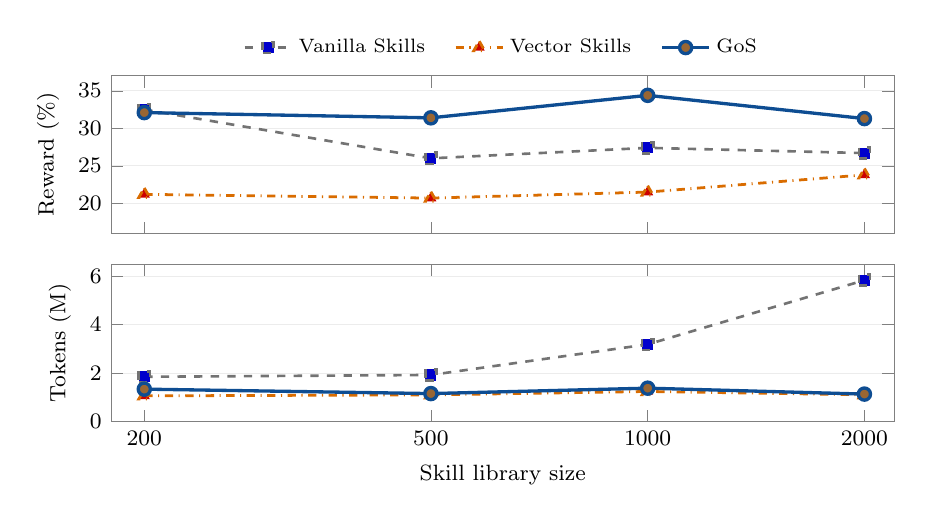
\begin{tikzpicture}

% 上方图表：Reward
\begin{axis}[
    name=plot1, 
    width=0.82\linewidth, % 【关键修改2】让出 12% 宽度给 Y 轴数字，防止超出页面边界
    height=2.0cm,         % 【关键修改3】高度压低至 1.4cm
    scale only axis, 
    xmode=log,
    log basis x=10,
    xmin=180, xmax=2200, 
    xtick={200,500,1000,2000}, 
    xticklabels=\empty, 
    ymin=16, ymax=37, 
    ymajorgrids=true,
    grid style={draw=gray!15},
    axis line style={draw=black!50},
    tick style={draw=black!50},
    label style={font=\footnotesize},
    tick label style={font=\footnotesize},
    ylabel={Reward (\%)},
    legend columns=3, 
    legend style={
        draw=none, fill=none, font=\scriptsize, 
        at={(0.5,1.05)}, anchor=south, 
        /tikz/every even column/.append style={column sep=0.3cm}
    },
    legend cell align=left,
]
\addplot+[color=black!55, mark=square*, dashed, line width=0.95pt, mark size=2pt] coordinates {(200,32.5) (500,26.0) (1000,27.4) (2000,26.7)};
\addplot+[color=orange!85!black, mark=triangle*, dashdotted, line width=1.0pt, mark size=2.3pt] coordinates {(200,21.2) (500,20.7) (1000,21.5) (2000,23.8)};
\addplot+[color=darkblue, mark=*, line width=1.2pt, mark size=2.2pt] coordinates {(200,32.1) (500,31.4) (1000,34.4) (2000,31.3)};
\legend{Vanilla Skills, Vector Skills, GoS}
\end{axis}

% 下方图表：Tokens
\begin{axis}[
    name=plot2,
    at={(plot1.below south west)}, 
    anchor=north west,
    yshift=-0.15cm,       % 稍微调整上下图间隙
    width=0.82\linewidth, % 【关键修改2】同上
    height=2.0cm,         % 【关键修改3】同上
    scale only axis, 
    xmode=log,
    log basis x=10,
    xmin=180, xmax=2200, 
    xtick={200,500,1000,2000},
    xticklabels={200,500,1000,2000}, 
    ymin=0, ymax=6.5,
    ymajorgrids=true,
    grid style={draw=gray!15},
    axis line style={draw=black!50},
    tick style={draw=black!50},
    label style={font=\footnotesize},
    tick label style={font=\footnotesize},
    xlabel={Skill library size},
    ylabel={Tokens (M)}, 
]
\addplot+[color=black!55, mark=square*, dashed, line width=0.95pt, mark size=2pt] coordinates {(200,1.850) (500,1.925) (1000,3.188) (2000,5.836)};
\addplot+[color=orange!85!black, mark=triangle*, dashdotted, line width=1.0pt, mark size=2.3pt] coordinates {(200,1.063) (500,1.102) (1000,1.244) (2000,1.106)};
\addplot+[color=darkblue, mark=*, line width=1.2pt, mark size=2.2pt] coordinates {(200,1.340) (500,1.157) (1000,1.380) (2000,1.136)};
\end{axis}
\end{tikzpicture}
\end{minipage}

\end{figure*}


\noindent\textbf{Prompt cost grows rapidly for all skill exposure.}
The strongest trend is on input tokens. 
%
As the library grows from 500 to 2,000 skills, \textit{Vanilla Skills} rises from 1.93M to 5.84M average input tokens, roughly a 3$\times$ increase. Over the same range, \textit{Vector Skills} stays near 1.10M--1.24M tokens and GoS stays near 1.14M--1.38M tokens. 
%
This result shows that simple retrieval substantially weakens the coupling between repository size and prompt size, while GoS does so without giving up reward.

\noindent\textbf{GoS maintains a reward advantage at all tested scales.}
At 200 skills, \textit{Vanilla Skills} is still slightly ahead of GoS (32.5 vs. 32.1). 
%
Once the library becomes moderately large, GoS outperforms both baselines at every tested scale: 31.4 vs. 26.0 / 20.7 at 500 skills, 34.4 vs. 27.4 / 21.5 at 1{,}000 skills, and 31.3 vs. 26.7 / 23.8 at 2{,}000 skills (GoS / Vanilla Skills / Vector Skills). The margin is largest at 1{,}000 skills and remains substantial at 2{,}000, indicating that increasing library size does not weaken the benefit of dependency-aware retrieval.

\noindent\textbf{Retrieval step does not change the scaling conclusion.}
Both retrieval-based methods are slower than \textit{Vanilla Skills} in agent-only runtime for GPT at most scales, reflecting the overhead of searching before execution. 
% However, that runtime overhead is modest relative to the reduction in prompt cost, and the main scaling bottleneck remains the prompt itself rather than retrieval latency. 
%
However, this reduced runtime is unique to GPT-5.2 Codex, likely due to caching mechanisms for fixed skill libraries within the black-box model, where Claude and MiniMax have longer runtime when using \textit{Vanilla Skills} than GoS and \textit{Vector Skills} (Table~\ref{results-table}).
%
In contrast, the Claude model lacks this optimization, making the \textit{Vanilla Skills} approach significantly slower than retrieval methods. 
%
Furthermore, the results suggest that the primary system bottleneck is not graph traversal or vector search, but rather the overhead of exposing an increasingly large, flat library directly to the model.
% The runtime pattern is summarized in Table~\ref{tab:claude_runtime_wrap}. These comparisons indicate that for Claude-style agents, retrieval not only reduces tokens but also yields a practical runtime advantage. 
% %
% \begin{wraptable}{r}{0.5\linewidth}
% % \vspace{-0.8em}
% % \centering
% \small
% \label{tab:claude_runtime_wrap}
% % \begin{tabular}{llll}
% % \toprule
% % Model & Method & S \\
% % \midrule
% % %  & Vanilla Skills & 465.8 & 53.22 \\
% % Claude 4.5 & Vector & \textbf{357.3} & \textbf{37.8} \\
% %  & +GoS & \underline{\underline{364.9}} & \underline{49.2}\\
% % \midrule
%  & Vanilla Skills & \underline{580.7} & 88.6\\
% % MiniMax M2.7 & Vector Skills & \underline{552.9} & \textbf{57.0} \\
% %  & +GoS & \textbf{502.5} & \underline{64.7} \\
% % \bottomrule
% % \end{tabular}
% % \vspace{-0.8em}
% % \end{wraptable}
% % Furthermore, this suggests that the primary system bottleneck is not graph traversal or vector search, but rather the overhead of exposing an increasingly large, flat library directly to the model.


% % This skillset size sensitivity study shows that GoS is not only stronger at the fixed 1{,}000-skill setting used in the main table; it is also more robust as the underlying skill repository grows. 
% % %
% As library size increases, the \textit{Vanilla Skills} baseline consumes increasing context cost without much reward gains, vector retrieval preserves compression but remains weaker on reward, and GoS preserves the most balanced overall contribution-efficiency key tradeoff.
% 
\subsection{Component Analysis of Retrieval Pipeline}
%%
\begin{table}[t]
\caption{Component ablation on full SkillsBench with GPT-5.2 Codex and the 1{,}000-skill library. \textbf{R}: average reward (\%), \textbf{T}: average total tokens (M), \textbf{S}: agent-only runtime (s).}
\label{tab:gos-ablation}
\centering
\footnotesize
\setlength{\tabcolsep}{4.5pt}
\begin{tabular}{lccc}
\toprule
Method & R $\uparrow$ & T $\downarrow$ & S $\downarrow$ \\
\midrule
Full GoS & \textbf{34.4} & 1.38 & 715.6 \\
w/o graph propagation & 29.3 & 0.89 & 766.2 \\
w/o lexical + rerank & 26.7 & 1.01 & 747.7 \\
\bottomrule
\end{tabular}
\end{table}

We next evaluate the contribution of two key retrieval components in the GoS pipeline: graph propagation and lexical reranking, with results reported in Table~\ref{tab:gos-ablation}.
%
These ablations were run under the main SkillsBench configuration with GPT-5.2 Codex on the 1{,}000-skill library.
%
In the first ablation, we remove graph propagation, disabling the system's ability to expand beyond seed skills to structurally related prerequisites. 
%
In the second, we remove lexical retrieval and reranking, forcing the system to rely solely on the semantic retriever before graph expansion.
%


\textbf{Graph propagation and lexical reranking are important components for GoS' success.}
%
Removing graph propagation reduces average token usage from 1.38M to 0.89M, but it also lowers average reward from 34.4 to 29.3 ($\downarrow5.1$). 
%
Removing lexical retrieval and reranking lowers average token usage from 1.38M to 1.01M. It lowers average reward from 34.4 to 26.7 ($\downarrow7.7$). 
%
The larger degradation in the second ablation suggests that better seed quality is especially important on SkillsBench: if the initial retrieved skills are weak, graph expansion has less useful structure from which to recover missing prerequisites.
% At the same time, graph propagation remains an important part of the final gain. Even with lexical retrieval and reranking intact, removing graph propagation still causes a substantial reward loss relative to the full system. Taken together, 
These results show that hybrid semantic--lexical retrieval improves entry-point quality, and graph propagation then converts those stronger seeds into a more execution-complete bundle. 
%

%


\section{Conclusion}
Skill retrieval is a critical bottleneck for agents over massive skill libraries: vanilla loading is expensive and noisy, while vector retrieval misses prerequisite chains.
%
GoS addresses both by retrieving a small, jointly sufficient bundle---target skill plus the parsers, preprocessors, and dependencies needed for execution.
%
On the 1{,}000-skill SkillsBench under GPT-5.2 Codex, GoS attains a peak reward gain of $25.55\%$ over the full-loading baseline while reducing total tokens by $56.72\%$, and improves over both baselines in every one of the six model--benchmark blocks spanning Claude Sonnet 4.5, MiniMax M2.7, and GPT-5.2 Codex.
%
The library-size study from 200 to 2{,}000 skills confirms this advantage holds as the library scales.



\section*{Limitations}

\noindent\textbf{Graph construction quality.} GoS depends on the quality of its offline skill graph. Poorly documented skills or ambiguous I/O schemas can degrade edge quality, and these errors propagate into retrieval.

\noindent\textbf{Static graph after construction.} The skill graph is built offline and is not updated from downstream execution traces or user feedback. As a result, GoS cannot self-correct when an induced dependency is wrong or when a useful relation was missed during construction.

\noindent\textbf{Evaluation scope.} Our evaluation covers two benchmarks (SkillsBench and ALFWorld) and three model families. We have not evaluated GoS on multimodal embodied agents, web-browsing agents, or other interactive settings where the operational notion of a skill may differ from the one studied here.


% \section*{Ethical Considerations} 
% This paper presents work whose goal is to advance the field of machine learning. There are no potential societal consequences of our work which we feel must be specifically highlighted here.

% \input{sections/reproducibility_statement}

% Custom bibliography entries only
\bibliography{custom}

\clearpage
\appendix

\section{Appendix Overview}

To make the supplementary material easier to navigate, we briefly summarize the organization of the appendix before presenting the detailed evidence. The appendix is designed to complement the main paper along four axes: implementation fidelity, prompt/interface design, retrieval mechanics, and trajectory-grounded empirical analysis.

\begin{table}[H]
\centering
\small
\caption{Appendix roadmap. The table summarizes the role of each supplementary section and how it complements the main paper.}
\label{tab:appendix_roadmap}
\begin{ApdxTabFrame}
\begin{tabular}{p{0.28\linewidth}p{0.62\linewidth}}
\toprule
\rowcolor{appendixolive}
\apdxhdr{Section} & \apdxhdr{Purpose} \\
\midrule
Implementation Details & Documents how GoS is instantiated in code, including parsing, graph construction, hybrid seeding, diffusion, reranking, and hydration. \\
Prompt and Interface Examples & Shows representative internal prompts and agent-facing interface rules used during graph construction and online retrieval. \\
Core Retrieval Pseudocode & Gives compact pseudocode for the offline indexing pipeline and the online graph-based retrieval pipeline. \\
Error Analysis & Separates retrieval misses, partial retrieval, execution drift, and infrastructure failures. \\
Qualitative Analysis & Provides trajectory-grounded case studies that compare the actual skill context exposed under different retrieval conditions. \\
\bottomrule
\end{tabular}
\end{ApdxTabFrame}
\end{table}

\section{Implementation Details}

This appendix summarizes the implementation decisions behind GoS and clarifies how the abstract pipeline in the main text is instantiated in code. The purpose is not to enumerate every engineering detail, but to expose the concrete design choices that determine graph quality, retrieval behavior, and the final agent-facing bundle.

\begin{table}[H]
\centering
\small
\caption{GoS implementation summary. The table highlights the main design choices that determine graph construction, retrieval, and agent-facing hydration.}
\label{tab:appendix_impl_summary}
\begin{ApdxTabFrame}
\begin{tabular}{p{0.23\linewidth}p{0.69\linewidth}}
\toprule
\rowcolor{appendixolive}
\apdxhdr{Component} & \apdxhdr{Implementation choice} \\
\midrule
Node construction & Parser-first normalization from \texttt{SKILL.md} plus optional LLM completion of retrieval-critical semantic fields. \\
Dependency edges & Directed edges induced by bidirectional output--input compatibility checks. \\
Higher-order edges & Sparse LLM validation over a bounded candidate pool for workflow, semantic, and alternative relations. \\
Seed retrieval & Hybrid semantic and lexical seeding over normalized node fields. \\
Graph scoring & Reverse-aware typed Personalized PageRank with relation-specific reverse transitions. \\
Final output & Reranked, budgeted hydration into agent-usable skill payloads with stable \texttt{Source:} paths. \\
\bottomrule
\end{tabular}
\end{ApdxTabFrame}
\end{table}

\begin{table*}[!t]
\centering
\small
\caption{Normalized node fields used at retrieval time. The table lists the fields retained in each skill node and their retrieval role in GoS.}
\label{tab:appendix_node_fields}
\begin{ApdxTabFrame}
\begin{tabular}{p{0.24\linewidth}p{0.22\linewidth}p{0.44\linewidth}}
\toprule
\rowcolor{appendixolive}
\apdxhdr{Field} & \apdxhdr{Primary role} & \apdxhdr{Why it matters} \\
\midrule
\texttt{name}, \texttt{description} & canonical identity and coarse semantic match & Provide the most stable high-level skill signature during lexical and semantic seeding. \\

\texttt{one\_line\_capability} & concise capability abstraction & Helps retrieval align a task to what the skill actually does, rather than to document wording alone. \\

\texttt{inputs}, \texttt{outputs} & executable interface schema & Support deterministic dependency induction and help retrieval recover prerequisite producers and consumers. \\

\texttt{domain\_tags}, \texttt{tooling} & technical context & Improve matching on domain-specific libraries, APIs, and workflows when task language is underspecified. \\

\texttt{example\_tasks} & usage priors & Improve recall for tasks described by objective or scenario rather than by direct tool names. \\

\texttt{script\_entrypoints} & implementation affordances & Help the agent discover reusable scripts instead of re-implementing logic from scratch. \\

\texttt{compatibility}, \texttt{allowed\_tools} & execution constraints & Preserve operational restrictions that are important for verifier-aligned use. \\

\texttt{source\_path}, \texttt{rendered\_snippet} & hydration and agent consumption & Make retrieved skills directly inspectable inside the execution environment and keep the bundle compact. \\
\bottomrule
\end{tabular}
\end{ApdxTabFrame}
\end{table*}

\begin{table*}[!t]
\centering
\small
\caption{Relation types and edge weights used in reverse-aware graph diffusion. Forward weights govern transition mass along the stored edge direction; reverse weights govern backward propagation from a matched skill toward its likely prerequisites. Dependency edges, the only deterministically induced relation, receive the largest weight in both directions; the three LLM-validated relations receive smaller reverse weights to limit topical drift during diffusion.}
\label{tab:appendix_relation_weights}
\begin{ApdxTabFrame}
\begin{tabular}{p{0.16\linewidth}p{0.10\linewidth}p{0.10\linewidth}p{0.22\linewidth}p{0.28\linewidth}}
\toprule
\rowcolor{appendixolive}
\apdxhdr{Relation} & \apdxhdr{Forward} & \apdxhdr{Reverse} & \apdxhdr{Meaning} & \apdxhdr{Retrieval consequence} \\
\midrule
Dependency & 1.0 & 1.0 & Skill $u$ produces an artifact consumed by skill $v$ & Strongest forward and backward propagation, since recovering prerequisites is the main purpose of GoS. \\

Workflow & 0.7 & 0.5 & Two skills are commonly chained in a concrete multi-step pipeline & Allows moderate backward expansion toward adjacent pipeline stages without dominating dependency evidence. \\

Semantic & 0.4 & 0.2 & Two skills belong to the same narrow capability cluster & Provides weak smoothing across near-neighbor skills while limiting topical drift. \\

Alternative & 0.3 & 0.1 & Two skills solve the same subproblem via different implementations & Provides minimal backward mass, mainly to keep interchangeable options reachable. \\
\bottomrule
\end{tabular}
\end{ApdxTabFrame}
\end{table*}

\begin{table*}[!t]
\centering
\small
\caption{GoS hyperparameters used in all reported experiments. Values are the defaults shipped in the released code and are held fixed across benchmarks, model families, and library sizes unless explicitly noted.}
\label{tab:appendix_hyperparams}
\begin{ApdxTabFrame}
\begin{tabular}{p{0.30\linewidth}p{0.10\linewidth}p{0.50\linewidth}}
\toprule
\rowcolor{appendixolive}
\apdxhdr{Hyperparameter} & \apdxhdr{Value} & \apdxhdr{Role} \\
\midrule
PPR restart $\alpha$ & 0.2 & Teleport probability in Eq.~\eqref{eq:ppr}; controls how much mass stays near the seeds. \\
PPR max iterations & 50 & Power-iteration cap for the diffusion in Eq.~\eqref{eq:ppr}. \\
PPR tolerance & $10^{-6}$ & Convergence threshold on $\lVert \mathbf{s}^{(\ell+1)} - \mathbf{s}^{(\ell)} \rVert$. \\
Dependency I/O threshold $\zeta$ & 0.6 & Minimum schema-overlap score required to add a deterministic dependency edge. \\
Validation candidates per node $k$ & 8 & Top-$k$ candidates per node sent to the LLM relation validator. \\
Semantic seed pool & 20 & Dense-retrieval candidate count per query before merging. \\
Lexical seed pool & 20 & Lexical-retrieval candidate count per query before merging. \\
Seed set size & 5 & Number of merged seeds carried into graph diffusion. \\
Retrieval top-$N$ & 8 & Maximum number of hydrated skills returned to the agent. \\
Per-skill char budget & 2{,}400 & Truncation limit applied to each hydrated skill payload. \\
Global context char budget & 12{,}000 & Total character budget over the hydrated bundle. \\
\bottomrule
\end{tabular}
\end{ApdxTabFrame}
\end{table*}

\begin{ApdxCallout}
\noindent\textbf{Pipeline Summary.}
GoS proceeds in two phases. Offline, it parses local skill packages into normalized nodes, adds dependency edges by I/O matching, and augments the graph with sparse workflow, semantic, and alternative relations. Online, it forms a hybrid semantic--lexical seed set, applies reverse-aware graph diffusion, and returns a reranked, budgeted bundle of execution-ready skills.
\end{ApdxCallout}

\paragraph{Implementation Substrate.}
GoS is implemented on top of a graph-backed retrieval substrate for workspace management, vector indexing, and graph storage, while replacing document-centric assumptions with skill-specific parsing, relation induction, and agent-oriented hydration. Concretely, the system maintains an HNSW vector index over skill representations together with a typed directed graph whose vertices are normalized skills and whose edges carry relation labels, directional semantics, and scalar weights. This yields a retrieval substrate in which semantic proximity and structural connectivity can be combined inside a single inference-time pipeline rather than treated as disjoint retrieval regimes.

\paragraph{Parser-First Skill Normalization.}
Each local \skillpackage{} is first parsed deterministically from its primary \texttt{SKILL.md} file and nearby package structure. The parser extracts the canonical name and description from YAML frontmatter, collects explicit input and output fields, recovers domain tags, tooling, example tasks, compatibility notes, and allowed tools from both frontmatter and markdown sections, and resolves script entrypoints by scanning the local \texttt{scripts/} directory when present. It also materializes a stable local source path and a rendered snippet used later for retrieval and hydration. This parser-first design keeps node construction anchored in executable package structure rather than relying entirely on free-form semantic extraction.

\paragraph{LLM-Assisted Semantic Completion.}
When package documentation is incomplete, GoS optionally performs a lightweight LLM pass over the full markdown body to recover retrieval-critical semantic fields, including capability summaries, inputs, outputs, domain tags, tooling, and example tasks. Importantly, this stage is constrained to normalize a single skill node and is not used to emit graph relations directly. In other words, the LLM here serves as a high-precision semantic completion module for node attributes rather than as an unconstrained graph-construction oracle. The inferred fields are then merged back with the deterministic parse, with the implementation favoring completed semantic fields only when they improve the retrieval representation.

\paragraph{Typed Node Representation.}
After normalization, each skill is serialized into a node record that stores both structured lists and compact textual views. Besides canonical descriptive fields, the node retains raw skill content, rendered snippets, script entrypoints, and a stable \texttt{Source:} path. This dual representation is operationally important: the graph and vector index operate over normalized fields, whereas the final agent-facing bundle requires concise but directly usable payloads that can be opened inside the execution environment without path reconstruction.

\paragraph{Directed Typed Relation Induction.}
The GoS graph is a typed directed graph rather than an undirected similarity graph. Dependency edges are induced deterministically by matching producer outputs against consumer inputs in both directions for each candidate pair. An edge $u \rightarrow v$ therefore has explicit executable semantics: $u$ can plausibly provide an artifact consumed by $v$. Because I/O compatibility is asymmetric in general, this dependency structure cannot be reduced to undirected similarity without losing the notion of prerequisite direction.

Non-dependency relations, namely \emph{workflow}, \emph{semantic}, and \emph{alternative}, are added through sparse LLM validation rather than dense all-pairs inference. For each node, GoS first forms a bounded candidate pool by combining lexical overlap, semantic neighbors from the vector index, and I/O-based candidate expansion. The LLM is then asked only to validate high-confidence relations inside this restricted pool. This two-stage design keeps graph construction tractable and biases the resulting graph toward precision rather than density.

\paragraph{Hybrid Seeding at Query Time.}
At retrieval time, GoS does not rely on vector search alone. The system first optionally rewrites the raw task request into a compact query schema containing the goal, operations, artifacts, constraints, and high-value keywords. Semantic seeding is then obtained from nearest-neighbor search in embedding space, while lexical seeding is computed from token overlap over normalized node fields such as name, capability, I/O descriptors, tooling, example tasks, entrypoints, and snippets. These candidate pools are merged and reranked before graph diffusion, so the graph is seeded by a hybrid entry set rather than by a single retriever. In practice, this detail matters because the quality of the initial seeds strongly influences whether later graph expansion can recover the correct prerequisite chain.

\paragraph{Reverse-Aware Structural Diffusion.}
Retrieval over the graph uses a Personalized PageRank-style diffusion operator constructed from the directed typed edges. The implementation first inserts forward transition mass along each stored edge, and then injects type-specific reverse transitions so that relevance can flow back from a matched high-level skill toward likely prerequisites. The reverse coefficients are largest for dependency edges and smaller for workflow, semantic, and alternative links, reflecting the fact that reverse traversal is most justified when recovering executable prerequisites. Operationally, this means the graph remains directed, but retrieval is explicitly reverse-aware. GoS therefore does not collapse the graph into an undirected graph; instead, it performs controlled backward propagation during scoring.

\paragraph{Reranking and Budgeted Hydration.}
The stationary graph score is not exposed to the agent directly. After diffusion, GoS reranks candidate skills by combining graph relevance with field-level query evidence, then hydrates only the top skills into an agent-facing bundle under both per-skill and global context budgets. Each hydrated payload includes a concise skill rendering, relevant execution notes, and the original local source path. The retrieval output therefore functions as a bounded execution context rather than a generic search-result list. This final budgeted hydration step is essential for preserving the efficiency advantage over flat all-skills loading while still presenting enough structure for downstream execution.

\paragraph{Section Summary.}
From an implementation perspective, GoS is best understood as a hybrid graph-construction and retrieval system: deterministic parsing and I/O matching provide a reliable executable backbone; optional LLM semantic completion improves node quality when documentation is incomplete; sparse LLM relation validation adds higher-order inter-skill structure; and reverse-aware graph diffusion converts a small hybrid seed set into a compact, more execution-complete bundle. These implementation choices are what instantiate the central claim of the paper that structural retrieval should recover not only relevant skills, but also the prerequisite context needed to use them effectively.

\section{Prompt and Interface Examples}

\paragraph{Layered Prompt Design.}
GoS uses two prompt layers with deliberately separated responsibilities. The first layer operates \emph{inside} the indexing and retrieval stack, where LLMs are used only for constrained normalization, optional query rewriting, and sparse relation validation. The second layer operates at the \emph{agent interface}, where the environment prompt tells the downstream agent when to call retrieval, how to interpret the returned bundle, and how strongly to prefer reuse over open-ended exploration. This separation is methodologically important. Graph-side prompts determine what semantic structure enters the retrieval substrate, whereas agent-side prompts determine whether that retrieved structure is converted into a verifier-aligned execution plan.

\paragraph{Presentation Goal.}
This section is not intended to enumerate full prompt templates. Instead, it exposes the narrow prompt fragments and interface rules that are most important for understanding the method. From a reviewer perspective, the key point is that GoS does not rely on unconstrained prompt engineering. The internal prompts are used to normalize or validate bounded objects, and the external interface is used to constrain downstream behavior once retrieval has occurred. Together, these prompts form an interface contract between offline graph construction and online execution.

\begin{table*}[t]
\centering
\small
\caption{Representative prompt and interface components in GoS. The table highlights the small set of prompt contracts that shape graph construction and downstream agent behavior.}
\label{tab:appendix_prompt_examples}
\setlength{\tabcolsep}{5pt}
\renewcommand{\arraystretch}{1.2}
\begin{ApdxTabFrame}[width=\textwidth]
\begin{tabular}{p{0.16\textwidth}p{0.18\textwidth}p{0.27\textwidth}p{0.27\textwidth}}
\toprule
\rowcolor{appendixolive}
\apdxhdr{Component} & \apdxhdr{Role} & \apdxhdr{Key constraint} & \apdxhdr{Intended effect} \\
\midrule
\textbf{Internal Prompt A}\\Skill semantic completion & Normalize one skill document into retrieval-critical fields. & Preserve canonical \texttt{name}/\texttt{description}; fill only node-local semantic fields; return an empty \texttt{edges} list. & Improve node quality when \texttt{SKILL.md} is incomplete while preventing relation hallucination. \\

\textbf{Internal Prompt B}\\Relation validation & Verify whether a bounded candidate pair should receive a typed edge. & Restrict outputs to \{dependency, workflow, semantic, alternative\}; preserve exact source/target names; emit nothing when uncertain. & Keep the graph sparse and precise instead of generating dense all-pairs links. \\

\textbf{Internal Prompt C}\\Query rewrite & Rewrite a raw request into a compact retrieval schema. & Extract \texttt{goal}, \texttt{operations}, \texttt{artifacts}, \texttt{constraints}, and \texttt{keywords} without redefining the task. & Improve seed-stage lexical and semantic coverage while preserving task intent. \\

\textbf{Agent Interface}\\Retrieval usage contract & Tell the downstream agent when retrieval must be called and how the returned bundle should be used. & Run \texttt{graphskills-query} first; read \texttt{Retrieval Status}; use exact \texttt{Source:} paths; prefer adapting retrieved scripts; prioritize verifier-minimal behavior. & Make retrieval operational immediately, so the bundle narrows search instead of serving as optional background context. \\
\bottomrule
\end{tabular}
\end{ApdxTabFrame}
\end{table*}

\paragraph{Internal Prompt A: Skill Semantic Completion.}
The semantic-completion prompt is intentionally narrow. It asks the model to normalize exactly one skill document and extract only retrieval-critical fields. In the implementation, the prompt explicitly preserves the canonical \texttt{name} and \texttt{description} when present, emphasizes high precision, and requires the returned \texttt{edges} list to be empty. This design reflects a conservative use of LLMs: the model is allowed to fill semantic gaps in node attributes, but not to invent graph structure. Operationally, this improves the quality of node representations used for indexing while avoiding a common failure mode in LLM-built graphs, namely relation over-generation. The prompt is therefore best understood as a constrained semantic completion module, not as a latent graph generator.

\paragraph{Internal Prompt B: Relation Validation.}
The relation-validation prompt is invoked only after GoS has formed a small candidate pool using lexical overlap, semantic neighbors, and I/O-based expansion. The prompt defines four edge types: \emph{dependency}, \emph{workflow}, \emph{semantic}, and \emph{alternative}. It also explicitly instructs the model to prefer sparse, high-precision edges, to emit nothing when uncertain, and to preserve exact skill names in the \texttt{source} and \texttt{target} fields. This makes the prompt function more like a relation verifier than a free-form graph generator. In practice, this design is important because it limits graph density and preserves the typed semantics later used during reverse-aware diffusion.

\begin{GosPromptBox}{Prompt excerpt: skill semantic completion}
1. Extract exactly one skill node from the document.
3. Infer only retrieval-critical fields: capability, inputs,
   outputs, domain_tags, tooling, example_tasks.
6. Use high precision. If uncertain, leave a field empty.
7. Do not invent relationships. Return an empty `edges` list.
\end{GosPromptBox}

This excerpt illustrates the central design principle of the internal extraction prompt: GoS uses the LLM as a constrained semantic normalizer, not as an unconstrained graph author. For the appendix, the important point is not merely that an LLM appears in the pipeline, but that the allowable output space is sharply restricted to node-local semantic completion.

\paragraph{Internal Prompt C: Query Rewrite.}
The optional query-rewrite prompt maps a raw task request to a compact retrieval schema with fields such as \texttt{goal}, \texttt{operations}, \texttt{artifacts}, \texttt{constraints}, and \texttt{keywords}. The prompt explicitly instructs the model not to invent benchmark-specific labels and to leave unclear fields empty. This is consistent with the retrieval objective in GoS: rewriting is used only to expose retrieval-critical technical terms such as file formats, APIs, protocols, and concrete operations. It is not intended to change the task itself. When rewriting is disabled or unavailable, the system falls back to deterministic lexical normalization, so query rewriting is a retrieval enhancement rather than a mandatory dependency. In other words, the prompt improves lexical and semantic coverage at the seed stage, but it is not allowed to redefine the problem.

\paragraph{Agent Interface Prompt.}
In the SkillsBench GoS environment, the agent is instructed to begin with a targeted retrieval query built from the task goal, artifact or format, operation or API, and verifier-critical constraints. The interface then forces the agent to read the retrieval status before continuing. A \texttt{NO\_SKILL\_HIT} response means the agent must explicitly acknowledge that no relevant skill was found and proceed without claiming skill use. A \texttt{SKILL\_HIT} response means the returned bundle should be treated as a narrowing device: the agent is told to use the returned local source paths, inspect scripts before implementing from scratch, and prioritize the shortest path to verifier pass. This interface design matters because the main quality difference is often not whether some relevant skill exists somewhere in the library, but whether the agent receives a compact, execution-ready bundle early enough to affect the trajectory. In that sense, the interface prompt is part of the method rather than a presentation detail.

\begin{GosPromptBox}{Prompt excerpt: agent-facing retrieval interface}
Before writing any code, run:
graphskills-query "goal + artifact/format + operation/API +
verifier-critical constraint"

- If Retrieval Status: NO_SKILL_HIT, proceed without claiming skill use.
- If Retrieval Status: SKILL_HIT, use retrieved skills only as constraints.
- Use the exact Source path already returned.
- Prefer adapting retrieved scripts over broader re-implementation.
\end{GosPromptBox}

This second excerpt shows that the agent-facing interface is itself part of the method. It does not merely expose a search command. It constrains when retrieval is called, how the returned bundle is interpreted, and how aggressively the downstream agent is allowed to branch away from authoritative local implementations. The resulting effect is to make retrieval operational rather than decorative: the bundle is meant to narrow the search space immediately, not merely provide optional background context.

\paragraph{Section Summary.}
Taken together, these examples show that prompt design in GoS is not generic scaffolding. The internal prompts constrain how semantic structure enters the graph; the external interface constrains how retrieved structure enters the agent's working context. The two layers therefore form an interface contract between offline graph construction and online agent execution. This contract is especially important in our setting because many failures are not pure retrieval misses, but retrieval-hit trajectories in which the agent still drifts unless the interface strongly biases it toward verifier-minimal reuse. The appendix evidence should therefore be read as support for a broader methodological claim: in graph-augmented agent systems, retrieval quality depends not only on what is indexed, but also on how the retrieved structure is exposed and behaviorally enforced downstream.

\section{Core Retrieval Pseudocode}

\paragraph{Presentation Goal.}
For completeness, we provide pseudocode for the two main algorithmic stages of GoS: offline graph construction and online structural retrieval. The presentation is intentionally close to the implementation, but abstracted enough to foreground the method rather than the surrounding engineering details.

\begin{algorithm}[t]
\caption{Offline graph construction for GoS}
\label{alg:gos_offline}
\begin{algobox}
\alginput{Local skill documents $\mathcal{C}$, optional LLM services, linking budget $k$}
\algoutput{Typed directed graph $G=(V,E)$ and vector index over normalized skills}
\algstep{Initialize empty node set $V$ and edge set $E$.}
\algstep{For each skill document $d \in \mathcal{C}$:}
\algindent{Parse YAML frontmatter and markdown structure from \texttt{SKILL.md}.}
\algindent{Extract deterministic fields: name, description, inputs, outputs, tags, tooling, \texttt{Source:} path, and script entrypoints.}
\algindent{If retrieval-critical semantic fields are incomplete, run constrained semantic completion to fill capability, inputs, outputs, and example tasks.}
\algindent{Serialize the result as a normalized skill node $v$ and add $v$ to $V$.}
\algstep{For each ordered pair of nodes $(u,v)$ in a bounded candidate pool:}
\algindent{Compute producer--consumer overlap between outputs of $u$ and inputs of $v$.}
\algindent{If overlap exceeds threshold, add typed dependency edge $u \rightarrow v$.}
\algstep{For each node $u$:}
\algindent{Form a sparse candidate set using lexical similarity, semantic neighbors, and I/O-based expansion.}
\algindent{Run constrained relation validation on this candidate set.}
\algindent{Add validated workflow, semantic, and alternative edges to $E$.}
\algstep{Build an embedding index over the normalized node representations.}
\algstep{Persist the typed graph, vector index, and retrieval metadata to the GoS workspace.}
\end{algobox}
\end{algorithm}

\begin{algorithm}[t]
\caption{Online graph-based skill retrieval}
\label{alg:gos_online}
\begin{algobox}
\alginput{Query $q$, prebuilt GoS workspace, retrieval budget $\tau$}
\algoutput{Bounded execution bundle $B(q)$}
\algstep{Optionally rewrite $q$ into a compact schema containing goal, operations, artifacts, constraints, and keywords.}
\algstep{Retrieve semantic seed candidates from the vector index.}
\algstep{Retrieve lexical seed candidates from normalized node fields.}
\algstep{Merge the candidate pools and construct a seed distribution $\mathbf{p}$.}
\algstep{Build a typed transition matrix over the graph.}
\algindent{Add forward transition mass for each stored edge.}
\algindent{Add relation-specific reverse mass, with the largest reverse coefficient on dependency edges.}
\algstep{Run reverse-aware Personalized PageRank until convergence to obtain graph scores $\mathbf{s}^{\star}$.}
\algstep{Rerank candidate skills using graph score plus direct field-level evidence from the query.}
\algstep{Hydrate the ranked skills into agent-facing payloads with exact \texttt{Source:} paths and concise execution notes.}
\algstep{Truncate the hydrated bundle under per-skill and global context budgets.}
\algstep{Return retrieval status, ranked bundle summary, bounded agent-facing context, and graph evidence among selected skills when it fits the budget.}
\end{algobox}
\end{algorithm}

\paragraph{Implementation Correspondence.}
Algorithm~1 corresponds to the parser-first normalization and relation-induction logic in the GoS implementation. Algorithm~2 corresponds to the retrieval path and the reverse-aware Personalized PageRank utilities. In practice, these stages additionally include engineering details such as workspace bootstrapping, embedding-dimension checks, source-path rewriting for containerized environments, and context clipping under hard character budgets. We omit those details from the pseudocode because they are not conceptually central, but they are nevertheless important for stable end-to-end deployment.

\section{Error Analysis}

\paragraph{Error Taxonomy.}
We distinguish retrieval-side errors from downstream execution failures, since these correspond to different limits of the overall system. A retrieval method can fail because it never surfaces the correct skill, because it retrieves an incomplete bundle that omits critical prerequisites, or because it produces a broadly adequate bundle that is subsequently misused by the downstream agent. Treating these failure modes separately is important for attributing gains correctly: GoS is designed to improve retrieval completeness, but it cannot by itself eliminate planning or execution failures once a bundle has already been provided. Across our trajectories, several of the most informative failures are not simple retrieval misses, but long-horizon search failures in which the correct general tool family is present and the agent still does not converge to a verifier-passing implementation.

\begin{table}[t]
\centering
\small
\caption{Primary error modes in GoS-style retrieval experiments. The table separates retrieval failures, downstream execution failures, and infrastructure issues.}
\label{tab:appendix_error_modes}
\begin{ApdxTabFrame}
\setlength{\tabcolsep}{4.5pt}
\renewcommand{\arraystretch}{1.2}
% Narrow third column caused bad header hyphenation; \rowcolor + booktabs leaves thin inter-column gaps—tighter \tabcolsep and ragged p-columns reduce both.
\begin{tabular}{@{}>{\raggedright\arraybackslash}p{0.20\linewidth}>{\raggedright\arraybackslash}p{0.40\linewidth}>{\raggedright\arraybackslash}p{0.32\linewidth}@{}}
\rowcolor{appendixolive}
\apdxhdr{Error type} & \apdxhdr{Typical symptom} & \makecell[l]{\textcolor{white}{\textbf{Whether helps}}} \\
\midrule
Retrieval miss & The correct skill exists in the library but is never surfaced, so the agent falls back to a from-scratch path. & Yes; better seed quality and graph completion can reduce this failure. \\
Partial retrieval & A topically relevant skill is retrieved, but a parser, setup routine, converter, or constraint-carrying prerequisite is absent. & Yes; this is the main failure mode GoS is designed to reduce. \\
Good retrieval, bad execution & The retrieved bundle is broadly adequate, but the agent still drifts, over-engineers, or mismatches the verifier. & Only indirectly; this is primarily a backbone or planning issue. \\
Infrastructure failure & Build, environment, or startup failures prevent a meaningful episode from occurring. & No; these are excluded from model-quality comparisons. \\
\bottomrule
\end{tabular}
\end{ApdxTabFrame}
\end{table}

\paragraph{Retrieval Misses.}
A retrieval miss occurs when the correct skill exists in the repository but is not surfaced at all. In this regime, the agent is forced onto a generic from-scratch path, so any downstream failure should be attributed primarily to the retriever rather than to execution drift. Misses typically arise when the query language does not overlap strongly with the skill description, when the task is phrased around a downstream objective but the critical skill is an upstream parser or setup utility, or when semantic retrieval overweights topical similarity relative to executable relevance. A representative example is \texttt{dapt-intrusion-detection}. In the failed GoS-style trajectory, the agent issued \texttt{graphskills-query} but did not recover \texttt{pcap-analysis}, instead receiving an irrelevant bundle that included items such as \texttt{dc-power-flow} and \texttt{dialogue-graph}. By contrast, the stronger baseline trajectory opened \texttt{pcap-analysis} and reused its tested helper code. The resulting difference in behavior is characteristic of a true retrieval miss: once the relevant analysis skill is absent, the task degrades into from-scratch implementation and fails the verifier.

\paragraph{Partial Retrieval.}
Partial retrieval is more subtle and often more important. Here, the retrieved bundle contains an obviously relevant high-level skill, but omits one or more prerequisite helpers needed for successful completion. In our setting, these missing items are often parsers, format converters, preprocessing utilities, setup routines, or constraint-carrying reference skills. This is precisely the regime in which graph-aware retrieval is intended to help: once a high-level skill is matched as a seed, reverse-aware propagation can recover supporting skills that are weak semantic matches to the raw query but strong structural neighbors in the skill graph. \texttt{earthquake-phase-association} illustrates the boundary of this idea. In the stronger all-skills trajectory, the agent assembled a coherent seismic stack including \texttt{gamma-phase-associator}, \texttt{obspy-data-api}, \texttt{seisbench-model-api}, and \texttt{seismic-picker-selection}, and the task passed. In the corresponding GoS case, the graph retrieval did bring in a partially relevant seismic bundle, but the resulting context was still less complete, and the task failed with reward $0.0$. This suggests that structural retrieval helps only when the recovered neighborhood is sufficiently complete to support the downstream pipeline, not merely when one or two domain-relevant skills are present.

\paragraph{Good Retrieval, Bad Execution.}
Some failures occur even when the retrieved bundle is broadly adequate. In these cases, the agent may still over-generalize the task, ignore a retrieved authoritative interface, implement unnecessary functionality, or fail to align with the verifier. These episodes matter because they bound what can be credited to retrieval alone. They also motivate the conservative agent-facing instructions used in our environments, which emphasize verifier-minimal solutions, direct use of returned local source paths, and avoidance of unnecessary branching. \texttt{energy-market-pricing} is a representative example: both all-skills and GoS had access to the relevant economic-dispatch / power-flow skill family and both eventually passed, but the all-skills trajectory required substantially more agent time before converging. This is not a retrieval miss; it is a difference in how efficiently a broadly adequate bundle is converted into a verifier-passing plan. Conversely, \texttt{adaptive-cruise-control} shows the opposite failure mode: the retrieved bundle included clearly relevant control skills such as \texttt{pid-controller}, \texttt{mpc-horizon-tuning}, \texttt{vehicle-dynamics}, and \texttt{simulation-metrics}, yet the run still finished with reward $0.0$. In that case the failure is better described as long-horizon execution drift or verifier mismatch rather than poor retrieval.

A related example is \texttt{dialogue-parser}. Multiple conditions had access to relevant task structure, yet only the strongest GoS trajectory converted that context into a full pass, while other conditions remained at partial reward. This again indicates that the dominant bottleneck was not the absence of any relevant skill at all, but how effectively the agent translated the available skill context into the exact output expected by the verifier.

\paragraph{Infrastructure Failures.}
Finally, a subset of observed failures are not retrieval failures at all, but infrastructure failures such as environment build issues, setup crashes, or startup timeouts before a substantive episode begins. These cases are methodologically important but conceptually distinct: they should be tracked for experiment hygiene and rerun logic, yet they should not be interpreted as evidence against the quality of the retrieval method or the underlying model. Representative examples include Docker / BuildKit failures such as \texttt{layer does not exist} on \texttt{dapt-intrusion-detection}, missing compiler toolchains for \texttt{obspy}-dependent tasks, and logging failures that leave some trials with incomplete session traces or null token fields. These episodes matter operationally because they require reruns and infrastructure fixes, but they are not evidence about the retrieval quality of GoS, vector retrieval, or all-skills. For this reason, we treat them as experiment-hygiene issues and exclude them from method-quality interpretation whenever possible.

\section{Qualitative Analysis}
\label{sec:appendix_qualitative}

\paragraph{Section Framing.}
We next examine a set of trajectory-grounded qualitative cases and compare the concrete skill evidence that actually entered the agent's working context in each condition. Table~\ref{tab:appendix_qualitative_retrieval} reports the skills that materially shaped each run: for GoS and Vector Skills, these are the skills surfaced by the retrieval call and then used downstream, while for \textit{Vanilla Skills} they are the skills the agent explicitly opened from the mounted library. This keeps the comparison grounded in executed trajectories rather than hypothetical retrieval quality.

Across the cases below, we focus on a single question: does the method expose a compact, execution-ready bundle early enough to change the trajectory? The main qualitative difference is often not whether a relevant skill exists somewhere in the repository, but whether the agent receives the right subset in a form that can be operationalized under the task budget.

\begingroup
\setlength{\tabcolsep}{3pt}
\renewcommand{\arraystretch}{1.12}
\newcommand{\qskill}[1]{\texttt{#1}}
\newcommand{\qcell}[1]{\parbox[t]{\linewidth}{\raggedright #1}}
\begin{table*}[t]
\centering
\scriptsize
\caption{Trajectory-grounded skill evidence from executed qualitative cases. \textsc{Useful} denotes skills that were clearly operationalized downstream; \textsc{Noisy} denotes retrieved or opened items that were tangential or not visibly used.}
\label{tab:appendix_qualitative_retrieval}
\begin{ApdxTabFrame}[width=\textwidth]
\begin{tabularx}{\textwidth}{>{\raggedright\arraybackslash}p{0.145\textwidth}>{\raggedright\arraybackslash}X>{\raggedright\arraybackslash}X>{\raggedright\arraybackslash}X}
\toprule
\rowcolor{appendixolive}
\apdxhdr{Task} & \apdxhdr{GoS Bundle} & \apdxhdr{Vanilla Bundle} & \apdxhdr{Vector Bundle} \\
\midrule
\qcell{\texttt{pedestrian-}\\\texttt{traffic-}\\\texttt{counting}} &
\qcell{\textsc{Useful} \qskill{gemini-count-in-video}; \qskill{multimodal-fusion}; \qskill{openai-vision}; \qskill{video-frame-extraction}\\\textsc{Noisy} \qskill{threat-detection}} &
\qcell{\textsc{Useful} \qskill{gemini-count-in-video}; \qskill{object\_counter}; \qskill{openai-vision}; \qskill{video-frame-extraction}\\\textsc{Noisy} \qskill{alfworld-heat-object-}\\\qskill{with-appliance}; \qskill{alfworld-object-locator}; broader noisy context} &
\qcell{\textsc{Useful} none\\\textsc{Noisy} \qskill{google-classroom-automation}; \qskill{rdkit}; \qskill{salesforce-service-cloud-}\\\qskill{automation}; \qskill{segmetrics-automation}} \\

\qcell{\texttt{flood-risk-}\\\texttt{analysis}} &
\qcell{\textsc{Useful} \qskill{flood-detection}; \qskill{nws-flood-thresholds}; \qskill{usgs-data-download}\\\textsc{Noisy} \qskill{time\_series\_anomaly\_detection}; \qskill{-21risk-automation}} &
\qcell{\textsc{Useful} \qskill{flood-detection}; \qskill{nws-flood-thresholds}; \qskill{usgs-data-download}} &
\qcell{\textsc{Useful} none\\\textsc{Noisy} \qskill{leverly-automation}; \qskill{scienceworld-room-navigator}; \qskill{text-to-speech}; broader noisy context} \\

\qcell{\texttt{travel-}\\\texttt{planning}} &
\qcell{\textsc{Useful} \qskill{search-accommodations}; \qskill{search-attractions}; \qskill{search-cities}; \qskill{search-driving-distance}; \qskill{search-restaurants}\\\textsc{Noisy} \qskill{search-flights}; \qskill{fjsp-baseline-repair-}\\\qskill{with-downtime-and-policy}} &
\qcell{\textsc{Useful} \qskill{search-accommodations}; \qskill{search-attractions}; \qskill{search-cities}; \qskill{search-restaurants}} &
\qcell{\textsc{Useful} \qskill{search-accommodations}; \qskill{search-attractions}; \qskill{search-cities}; \qskill{search-driving-distance}; \qskill{search-restaurants}\\\textsc{Noisy} additional noisy items} \\

\qcell{\texttt{dapt-}\\\texttt{intrusion-}\\\texttt{detection}} &
\qcell{\textsc{Useful} \qskill{pcap-analysis}; \qskill{pcap-triage-tshark}\\\textsc{Noisy} \qskill{dc-power-flow}; \qskill{power-flow-data}; \qskill{-21risk-automation}} &
\qcell{\textsc{Useful} no clearly reused core skill} &
\qcell{\textsc{Useful} none\\\textsc{Noisy} \qskill{codacy-automation}; \qskill{jakarta-namespace}; \qskill{rootly-automation}; broader noisy context} \\

\qcell{\texttt{dialogue-}\\\texttt{parser}} &
\qcell{\textsc{Useful} \qskill{dialogue\_graph}; \qskill{webshop-query-parser}\\\textsc{Noisy} \qskill{browser-testing}; \qskill{obj-exporter}; \qskill{alfworld-goal-interpreter}} &
\qcell{\textsc{Useful} \qskill{dialogue\_graph}} &
\qcell{\textsc{Useful} none\\\textsc{Noisy} \qskill{docnify-automation}; \qskill{scienceworld-task-focuser}; \qskill{temporal-python-testing}; broader noisy context} \\

\qcell{\texttt{earthquake-}\\\texttt{phase-}\\\texttt{association}} &
\qcell{\textsc{Useful} \qskill{gamma-phase-associator}; \qskill{seisbench-model-api}; \qskill{seismic-picker-selection}\\\textsc{Noisy} \qskill{flood-detection}; \qskill{-21risk-automation}} &
\qcell{\textsc{Useful} \qskill{gamma-phase-associator}; \qskill{obspy-data-api}; \qskill{obspy-datacenter-client}; \qskill{seisbench-model-api}; \qskill{seismic-picker-selection}\\\textsc{Noisy} \qskill{gamma-automation}; \qskill{seismic-automation}} &
\qcell{\textsc{Useful} none\\\textsc{Noisy} \qskill{fixer-automation}; \qskill{maven-build-lifecycle}; \qskill{segmetrics-automation}; broader noisy context} \\

\qcell{\texttt{energy-}\\\texttt{market-}\\\texttt{pricing}} &
\qcell{\textsc{Useful} \qskill{dc-power-flow}; \qskill{power-flow-data}; \qskill{locational-marginal-}\\\qskill{prices}; \qskill{casadi-ipopt-nlp}\\\textsc{Noisy} \qskill{-21risk-automation}} &
\qcell{\textsc{Useful} \qskill{dc-power-flow}; \qskill{economic-dispatch}} &
\qcell{\textsc{Useful} \qskill{power-flow-data}\\\textsc{Noisy} \qskill{aryn-automation}; \qskill{moxie-automation}; \qskill{mural-automation}; broader noisy context} \\

\qcell{\texttt{3d-scan-}\\\texttt{calc}} &
\qcell{\textsc{Useful} \qskill{mesh-analysis}; \qskill{dyn-object-masks}\\\textsc{Noisy} \qskill{scienceworld-circuit-builder}; \qskill{scienceworld-circuit-}\\\qskill{connector}; \qskill{scienceworld-conductivity-}\\\qskill{tester}} &
\qcell{\textsc{Useful} \qskill{mesh-analysis}\\\textsc{Noisy} broader noisy context} &
\qcell{\textsc{Useful} \qskill{mesh-analysis}; \qskill{obj-exporter}; \qskill{pymatgen}; \qskill{threejs}\\\textsc{Noisy} \qskill{reflow-profile-compliance-}\\\qskill{toolkit}} \\

\qcell{\texttt{adaptive-}\\\texttt{cruise-}\\\texttt{control}} &
\qcell{\textsc{Useful} \qskill{imc-tuning-rules}; \qskill{pid-controller}; \qskill{safety-interlocks}; \qskill{vehicle-dynamics}\\\textsc{Noisy} \qskill{-21risk-automation}} &
\qcell{\textsc{Useful} no clearly reused core skill} &
\qcell{\textsc{Useful} \qskill{pid-controller}; \qskill{mpc-horizon-tuning}; \qskill{integral-action-design}; \qskill{simulation-metrics}; \qskill{vehicle-dynamics}} \\

\qcell{\texttt{econ-}\\\texttt{detrending-}\\\texttt{correlation}} &
\qcell{\textsc{Useful} \qskill{timeseries-detrending}\\\textsc{Noisy} \qskill{artifacts-builder}; \qskill{dyn-object-masks}; \qskill{mesh-analysis}; \qskill{-21risk-automation}} &
\qcell{\textsc{Useful} no clearly reused core skill} &
\qcell{\textsc{Useful} none\\\textsc{Noisy} \qskill{breezy-hr-automation}; \qskill{scienceworld-object-}\\\qskill{classifier}; \qskill{webshop-purchase-}\\\qskill{initiator}; broader noisy context} \\
\bottomrule
\end{tabularx}
\end{ApdxTabFrame}
\end{table*}
\endgroup

\paragraph{Case Study 1: Pedestrian Traffic Counting.} The clearest intermediate case in our trajectories is \texttt{pedestrian-traffic-counting}. The task requires frame extraction, reliable pedestrian counting, and structured output generation. GoS surfaced a compact visual pipeline centered on \texttt{gemini-count-in-video}, \texttt{video-frame-extraction}, and \texttt{openai-vision}, and achieved the strongest outcome among the three conditions ($0.417$). The \textit{Vanilla Skills} baseline did eventually open relevant helpers, including \texttt{gemini-count-in-video}, \texttt{video-frame-extraction}, and \texttt{object\_counter}, but reached only a partial score ($0.267$). The \textit{Vector Skills} run performed worst ($0.041$): although it issued the retrieval call, the retrieved context was not converted into a workable plan. This example is useful because it is not a pure pass/fail contrast. \textit{Vanilla Skills} does locate relevant functionality, but GoS exposes a smaller and more coherent bundle that appears easier to operationalize within the available task budget.

\paragraph{Case Study 2: Flood Risk Analysis.} The \texttt{flood-risk-analysis} task illustrates a different regime: both GoS and \textit{Vanilla Skills} succeed, but GoS exposes the required chain with much less search friction. In this task the correct workflow is not generic time-series analysis; it is specifically the combination of \texttt{usgs-data-download} for measurements, \texttt{nws-flood-thresholds} for stage cutoffs, and \texttt{flood-detection} for aggregation and comparison. GoS surfaced exactly this bundle and passed with reward $1.0$. The \textit{Vanilla Skills} baseline also passed with reward $1.0$, but only after the agent explicitly searched through the large mounted library and opened the same family of skills. \textit{Vector Skills}, by contrast, issued the retrieval command but never translated retrieval into a usable flood-analysis bundle, and the run failed with reward $0.0$. This case is useful because it does not primarily show a reward gap between GoS and \textit{Vanilla Skills}; instead, it shows that when the right execution chain exists in the repository, GoS mainly helps by making that chain explicit earlier in the trajectory.

\paragraph{Case Study 3: Travel Planning.} The \texttt{travel-planning} task is informative precisely because all three conditions surfaced clearly relevant travel skills. In the GoS run, the retrieved context centered on \texttt{search-cities}, \texttt{search-accommodations}, \texttt{search-attractions}, \texttt{search-driving-distance}, and \texttt{search-restaurants}, which is very close to the intended tool chain for the task. The \textit{Vanilla Skills} baseline likewise opened essentially the same family of skills after searching through the library. \textit{Vector Skills} also surfaced and used this same cluster of \texttt{search-*} skills, and that run passed the verifier with reward $1.0$. This example sharpens the qualitative claim of the paper. The advantage of GoS is not that flat semantic retrieval can never recover the correct skill family; rather, it is that GoS more reliably exposes a compact and coherent bundle early in the episode. When \textit{Vector Skills} does succeed, as it does here, its behavior becomes qualitatively much closer to GoS than to a clean retrieval miss.

\paragraph{Case Study 4: Network Intrusion Detection.} A clean GoS-positive example is \texttt{dapt-intrusion-detection}. In this case, GoS surfaced \texttt{pcap-analysis} together with adjacent analysis helpers such as \texttt{pcap-triage-tshark} and \texttt{threat-detection}, and the task passed. By contrast, the corresponding vector condition retrieved unrelated automation-oriented skills rather than a usable PCAP analysis bundle, while the all-skills condition still failed despite full library access. This case is a useful counterpart to the retrieval-miss pattern discussed in the Error Analysis section: once retrieval surfaces the right analysis bundle, the task becomes a reuse problem rather than a from-scratch reverse-engineering problem.

\paragraph{Case Study 5: Dialogue Parsing.} The \texttt{dialogue-parser} examples show a strong gradient across methods. GoS converted the task into a full pass while exposing a compact bundle centered on \texttt{dialogue\_graph}, together with structural helpers such as \texttt{obj-exporter}, \texttt{browser-testing}, and parser-oriented support. \textit{Vanilla Skills} eventually improved once it explicitly opened \texttt{dialogue\_graph}, and \textit{Vector Skills} also reached a substantial partial score, but neither condition showed the same level of structured completeness as the strongest GoS trajectory. This case illustrates a pattern that appears repeatedly: once the right latent-representation skill is surfaced early, the rest of the pipeline becomes much easier for the agent to operationalize.

\paragraph{Case Study 6: Earthquake Phase Association.} \texttt{earthquake-phase-association} is a useful negative case for GoS because it shows that structural retrieval does not help automatically when the recovered neighborhood is still incomplete. In the strongest all-skills trajectory, the agent assembled a seismic processing stack including \texttt{gamma-phase-associator}, \texttt{obspy-data-api}, \texttt{obspy-datacenter-client}, \texttt{seisbench-model-api}, and \texttt{seismic-picker-selection}, and the task passed. The corresponding GoS case surfaced only a weaker subset, centered on \texttt{gamma-phase-associator}, \texttt{seisbench-model-api}, and \texttt{seismic-picker-selection}, with an irrelevant distraction skill mixed into the bundle, and the task failed. This is exactly the kind of case that is easy to miss if one looks only at whether some domain-relevant skill was retrieved. The qualitative difference is that the all-skills trajectory assembled a more execution-complete stack, while the GoS trajectory remained one step short of the required pipeline.

\paragraph{Case Study 7: Energy Market Pricing.} A final useful case is \texttt{energy-market-pricing}, where all-skills and GoS both passed but with very different trajectory quality. The all-skills condition explicitly used \texttt{dc-power-flow} and \texttt{economic-dispatch}, while GoS surfaced a broader but still coherent optimization bundle including \texttt{dc-power-flow}, \texttt{power-flow-data}, \texttt{locational-marginal-prices}, and \texttt{casadi-ipopt-nlp}. Both runs eventually passed the verifier, but the trajectory quality differed sharply: GoS converted the retrieved bundle into a solution with substantially less agent-side search. This is one of the clearest examples in which the main value of GoS is not higher reward, but a shorter path from retrieval to execution.

\paragraph{Case Study 8: 3D Scan Calculation.} The \texttt{3d-scan-calc} task serves as a useful control because all three conditions can succeed when they recover the same latent geometry bottleneck. GoS exposed \texttt{mesh-analysis} together with adjacent geometric helpers, directly matching the preprocessing structure of the task. \textit{Vanilla Skills} also reached a passing solution once the agent opened \texttt{mesh-analysis}, but the surrounding library context was notably noisier. \textit{Vector Skills} likewise passed when it surfaced \texttt{mesh-analysis} together with geometry-oriented companions such as \texttt{obj-exporter}, \texttt{pymatgen}, and \texttt{threejs}. The qualitative lesson is therefore not that GoS is uniquely capable of solving the task; rather, when all methods recover a geometry-centered bundle, all can succeed, and the remaining difference is how directly that bundle is exposed.

\paragraph{Case Study 9: Adaptive Cruise Control.} \texttt{adaptive-cruise-control} is a useful failure case because all three conditions surfaced highly plausible control-related skills and still failed. GoS exposed \texttt{imc-tuning-rules}, \texttt{pid-controller}, \texttt{safety-interlocks}, and \texttt{vehicle-dynamics}, while \textit{Vector Skills} surfaced an even more explicit control bundle including \texttt{pid-controller}, \texttt{mpc-horizon-tuning}, \texttt{integral-action-design}, \texttt{simulation-metrics}, and \texttt{vehicle-dynamics}. The \textit{Vanilla Skills} condition also had access to a broad control-oriented context, yet none of the three settings converged to a passing solution. This case is important precisely because it is not a retrieval miss. It shows that once the task requires a long control-design and verifier-alignment chain, even a qualitatively good skill bundle may not be enough; the dominant bottleneck shifts from retrieval to execution discipline.

\paragraph{Case Study 10: Economic Detrending and Correlation.} The \texttt{econ-detrending-correlation} task offers a complementary success case. GoS surfaced \texttt{timeseries-detrending} and converted the task into a full pass, while the all-skills condition failed to assemble a comparably coherent detrending-centered bundle. \textit{Vector Skills} also reached a full pass, but with a noisier retrieved context whose skills were only weakly connected to the intended econometric workflow. This case is useful in two ways. First, it shows another task where surfacing the right latent preprocessing step, here detrending rather than raw correlation, materially changes the result. Second, it reinforces the lesson from \texttt{travel-planning}: vector retrieval can still succeed, but its successful episodes do not always arise from a bundle that is as semantically crisp or structurally interpretable as the one surfaced by GoS.

\paragraph{Takeaway.} Across all ten qualitative cases in this appendix, the main pattern is not simply that GoS retrieves skills with better topical overlap. Rather, GoS more often exposes a bundle that is already close to the executable decomposition of the task. The \texttt{pedestrian-traffic-counting} example shows a genuine middle case in which \textit{Vanilla Skills} finds relevant tools but still underperforms the tighter GoS bundle. The \texttt{flood-risk-analysis} example shows that when the correct chain is available to multiple methods, GoS mainly reduces search friction and makes the intended execution path explicit earlier. The \texttt{travel-planning}, \texttt{3d-scan-calc}, and \texttt{econ-detrending-correlation} examples show that \textit{Vector Skills} can also succeed when it recovers the right family of skills, but these successes are most convincing when the retrieved bundle becomes qualitatively similar to what GoS surfaces directly. The \texttt{dialogue-parser} and \texttt{dapt-intrusion-detection} cases show how GoS can convert that structural advantage into clearer downstream wins. By contrast, \texttt{earthquake-phase-association} shows a real boundary condition in which GoS still falls short of an execution-complete bundle, while \texttt{energy-market-pricing} and \texttt{adaptive-cruise-control} show that even with broadly adequate retrieval, trajectory efficiency and verifier alignment remain separate bottlenecks. Taken together, these cases support the core claim of the paper: structural retrieval helps not only by improving relevance, but by presenting agents with a more execution-ready context.


\end{document}
